\documentclass[a4paper]{book}

\usepackage[parts]{classicthesis}

\title{\textsf{Supervised Machine Learning techniques for quench detection in superconductors}}
\author{Alessandro Biagiotti}
\date{Academic Year 2023/2024}

\usepackage{mqd}

\begin{document}

\frontmatter

\maketitle

\tableofcontents

\mainmatter

\setcounter{chapter}{-1}
\chapter{introduction}
This thesis was born as a cooperation between the department of Computer Science and Physics of
Milan University in an attempt of confirming or giving us a good reason to doubt the analytical
method originally found by Samuele Mariotto in his research on the localization of quench events for
the High Order Correctors superconducting magnets that will be mounted on the LHC experiment for the
HiLumi upgrade.

In the following I will be explaining some of the studies and results obtained in the field of
quench event recognition and quench event localization by using machine learning models to abstract
patterns from the measurements of magnetic field harmonics captured by Mariotto during his own
experiments.

In this document I chose to approach the matter as follows:
\begin{description}
	\item[\Cref{chp:soupcond-quench}] gives an overview of superconductivity and quench on a
		theoretical level.
	\item[\Cref{chp:ml}] gives an overview of the various models that have been used in the
		project on a theoretical level.
	\item[\Cref{chp:problem}] explains the challenges associated with the project, the datasets
		that have been used and the various testing and model selection procedures.
	\item[\Cref{chp:qrp}] introduces the Quench Recognition Problem, as well as the models
		utilized to solve the problem and the results obtained.
	\item[\Cref{chp:qlp}] introduces the Qench Localization Problem, the extension of previously
		obtained models to this new instance, and the final results.
	\item[\Cref{chp:future}] lists other ideas that came along while designing a solution for
		the two problems at hand.
	\item[\Cref{chp:conclusion}] closes the document with a couple of thoughts on the design and
		development process.
\end{description}

\chapter{Superconductivity and quench: an overview}
\label{chp:soupcond-quench}
In this chapter I will explain the very basic concepts of superconductivity and
superconductor quench applied to the field of superconducting magnets for particle accelerators.
\section{Superconductivity in theory}
\label{sec:soupcond}
Electronic motion in metallic or insulating materials is a very well studied and documented
phenomenon. Electrons passing through any material, endure a varying amount of disturbance based on
the type and structure of the material, this disturbance is known as electrical resistivity $\rho$. Given a
sample of a material of length $l$, cross-section $A$ and electrical resistance $R$, which is a
measure of its opposition to the flow of electric current, electrical resistivity can be computed
as:
\begin{equation}
	\label{eq:resistivity-cable}
	\rho = \frac{RA}{l} = \frac{m}{ne^2\tau}
\end{equation}
As highlighted in the second part of the equation, the resistivity of a material can be seen as a function of:
\begin{itemize}
	\item The mass of the electron $m$,
	\item The charge density $n$ of the material lattice,
	\item The charge of the electron $e$,
	\item The \emph{relaxation time} of the electron, which is the time interval occurring between two
	      successive electronic collisions $\tau$.
\end{itemize}
This other formulation allows us to interpret the resistivity based on the amount of electronic
interactions registered within the sample. The higher the number of interactions, the lower the
relaxation time, the higher the resistivity of the material.

Based on their value of resistivity, materials can be divided between metals and insulators. Metals
have a very low value of resistivity (usually less than $10^{-5}\Omega\cdot m$), while insulators impede the
flow of electric current. The resistivity for any sample of material can be described also as a
function of the temperature, if we suppose that its resistivity was measured at a reference
temperature $T_0$ and one is interested in the resistivity at a certain temperature $T$, it's
possible to link the resistivity at temperature $T$, $\rho_T$, to the reference resistivity,
$\rho_0$ and the temperature change $T - T_0$ multiplied by a regularization term.
\begin{equation}
	\label{eq:resistivity-func-of-temp}
	\rho_T = \rho_0[1 + \alpha(T - T_0)]
\end{equation}
$\alpha$ is known as the temperature coefficient of resistance, which is commonly defined as the
change in electrical resistance per degree of temperature change. Usually, pure metals have a
positive value of $\alpha$: copper, for instance, has $\alpha \approx 0.004\C^{-1})$; alloys can be
created to have coefficients close to $0\C^{-1}$. As a general rule of thumb, whenever the
temperature increases the resistivity of a metal increases, this is not necessarily
true for insulators. Thermal breakdown for insulators is a similar phenomenon to electrical
breakdown (the voltage reaches a critical level and the dielectric behaves like a normal conductor,
whenever we see a lightning we are experiencing electrical insulator breakdown, where the insulator
is air), if the temperature is too high the insulator breaks down and behaves like a normal conductor. A thorough description of the phenomenon is given in~\cite{kuvyrkin2022}

Superconductors are metals that follow classical thermodynamic properties when the temperature is
kept around ambient temperature. Their properties change drastically once the temperature gets
extremely close to $0$\K~\footnote{
	There are many different materials nowadays, known as High Temperature
	Superconductors, which have a critical temperature well above $0$\K, in this thesis though we will
	only be considering classic superconductors like $NbTi$.
}.

In 1911~\cite{invention-superconductivity} Kammerligh Onnes discovered that if a sample of mercury was cooled
until it reached the temperature of $4.2$\K, electrical resistance shown by the sample disappeared
sharply from a finite, measurable, value, as can be seen in \Cref{img:mercury-resistance}, reaching
a new state of matter called \emph{superconducting state}.
\begin{figure}[!ht]
	\centering
	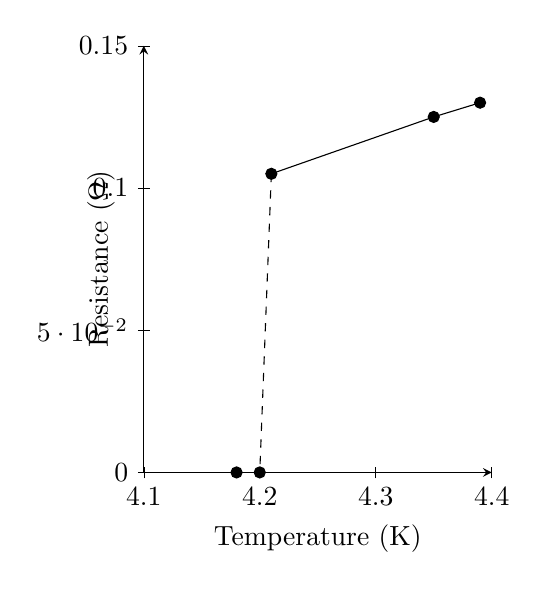
\begin{tikzpicture}
	\begin{axis}[
			width=6cm,
			height=7cm,
			xlabel={Temperature (K)},
			ylabel={Resistance ($\Omega$)},
			y label style = {at={(axis description cs:-0.055555,.5)},anchor=south},
			xmin=4.1,
			xmax=4.4,
			ymin=0,
			ymax=0.15,
			axis lines=left,
			tick style={black},
			no markers,
			samples=5
		]
		% Data points
		\addplot[only marks, mark=*] coordinates {
				(4.18, 0.000009)
				(4.20, 0.00001)
				(4.21, 0.105)
				(4.35, 0.125)
				(4.39, 0.130)
			};

		% Interpolation line
		\addplot[mark=*] coordinates {
				(4.21, 0.105)
				(4.35, 0.125)
				(4.39, 0.130)
			};

		\addplot[dashed, mark=*] coordinates {
				(4.21, 0.105)
				(4.20, 0.00001)
			};
	\end{axis}
\end{tikzpicture}

	\caption{The resistance of Mercury in function of the temperature of the sample, taken from~\cite{tsukerman2020compendium}}
	\label{img:mercury-resistance}
\end{figure}

Later studies discovered that many materials, pure and alloy, could be brought to the
superconducting state as long as three conditions were met:
\begin{itemize}
	\item The temperature of the sample didn't exceed the critical temperature $\tc$,
	\item The current density flowing in the sample didn't exceed the critical current
	      density $\jc$,
	\item The magnetic field acting on the material didn't exceed the critical magnetic field $\bc$.
\end{itemize}

When a material reaches the superconducting state it exhibits perfect diamagnetism, which means that
the material is able to perfectly expel the magnetic field lines from its volume (a simple experimental proof of this effect
is given by the magnetic levitation effect). This capacity was first observed by
Meissner and Ochsenfeld in 1933~\cite{meissner1933}. In 1935 the London's equations tried to explain
exotic behavior of different superconductor alloys which, in some situations, do not exhibit a perfectly diamagnetic behavior and allow the
penetration of external magnetic field lines down to a certain depth, known as the London's
penetration depth~\cite{london1935}. This property of superconductors was actually already theorized by Dutch
physicist Geertruida de Haas-Lorentz, who published some preliminary research in~\cite{fokker1925physica}.

The diamagnetic properties of superconductors depend heavily on the material microscopic properties. Two different Types of superconductors have been
identified and studied~\footnote{
	In general superconductor behavior can be explained through
	Ginzburg-Landau theory~\cite{Cyrot1973} but very recent research has proven that not every
	superconductor can be described using the \textsc{gl} equation as shown
	in~\cite{diamantini2023typeiiisuperconductivity}, this lead to the preliminary definition of
	a new type of superconductor, but, due to how recent the research is, it seems that, at the
	time of writing, nobody other than Diamantini published in the field of Type III superconductivity.
}, in the following I will provide a brief description of each.

\section{Type I superconductors}
\label{sec:type1}
\Cref{img:type1-transition}, plots magnetization, measuring the amount of induced or
permanent magnetic dipole moment of a magnet per unit volume~\cite{polarization-magnetization},
against external magnetic field $B$, applied on the sample. Once the magnetic field reaches $\bc$ the
magnetization of Type I superconductors drops to $0$.
\begin{figure}[!ht]
	\centering
	\begin{tikzpicture}
	% Axes
	\draw[->] (0,0) -- (5,0) node[right] {Applied Magnetic Fields, $B$};
	\draw[->] (0,0) -- (0,4) node[above] {Magnetization, $-M$};

	% Critical field B_c
	\node[below] at (3,0) {$B_c$};

	% Plot lines
	\draw[thick] (0,0) -- (3,3) -- (3,0);
\end{tikzpicture}

	\caption{Magnetization of a superconducting coil plotted against the external magnetic
		field, reproduction of the original plot taken from~\cite{slimani2022superconducting}}
\end{figure}
As long as the applied magnetic field is less than $\bc$, Type I superconductors exhibit perfect
diamagnetism, but once the material undergoes a transition to the normal-conducting
state (which will be referred to as \emph{quench} from now on) the magnetic dipole exerted by the
superconductor falls to zero (or a negligible value) allowing magnetic field penetration and making
such materials unsuitable for environments where a high magnetic field is required, such as fusion
reactors or particle physics experiments.

\section{Type II superconductors}
\label{sec:type2}
Type II superconductors, in most cases, are metal alloys. The characteristical impurity gives Type II superconductors an edge
over Type I, for high-field applications, due to the graceful degradation of magnetization with the increase in applied magnetic
field. A plot similar to \Cref{img:type1-transition} can be seen in \Cref{img:type2-transition}.
\begin{figure}[!ht]
	\centering
	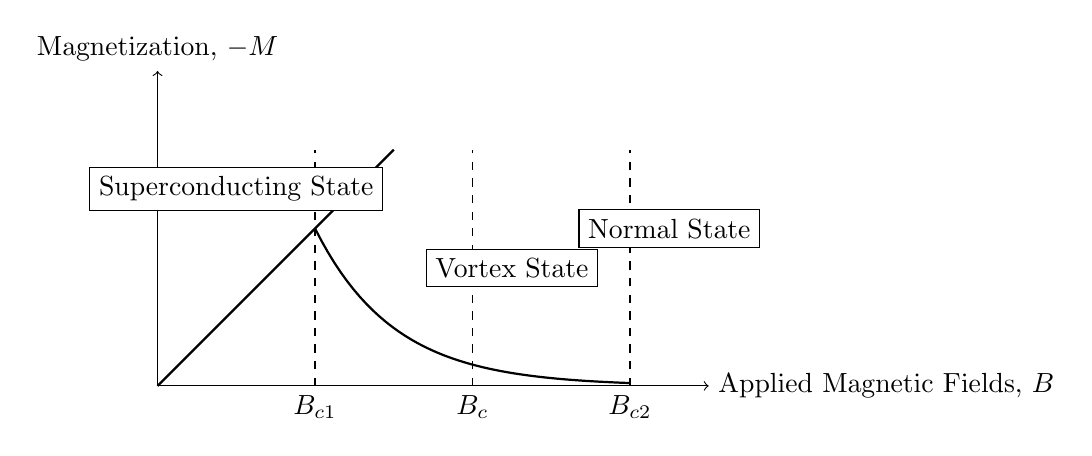
\begin{tikzpicture}
	% Axes
	\draw[->] (0,0) -- (7,0) node[right] {Applied Magnetic Fields, $B$};
	\draw[->] (0,0) -- (0,4) node[above] {Magnetization, $-M$};

	% Critical field labels
	\node[below] at (2,0) {$B_{c1}$};
	\node[below] at (4,0) {$B_c$};
	\node[below] at (6,0) {$B_{c2}$};

	% Dashed lines for critical fields
	\draw[dashed] (2,0) -- (2,3);
	\draw[dashed] (4,0) -- (4,3);
	\draw[dashed] (6,0) -- (6,3);

	% Magnetization curve
	\draw[thick] (0,0) -- (3,3);
	\draw[thick, domain=2:6, samples=50] plot (\x, {2*exp(-(\x-2))});

	% State labels with rectangles
	\node[draw, fill=white] at (1,2.5) {Superconducting State};
	\node[draw, fill=white] at (4.5,1.5) {Vortex State};
	\node[draw, fill=white] at (6.5,2) {Normal State};

\end{tikzpicture}

	\caption{Magnetization of a type II superconducting coil plotted against the external
		magnetic field, reproduction of the original plot taken from~\cite{slimani2022superconducting}}
	\label{img:type2-transition}
\end{figure}

Type II superconductors, while the applied magnetic field is less than $B_{C1}$, have the same
diamagnetic properties of Type I superconductors. Once the applied magnetic field surpasses the
$B_{C1}$ threshold, instead of having a very sharp transition from the superconducting state to
the normal-conducting state, these materials remain in an intermediate state referred to as the \emph{vortex} or \emph{hybrid state}.

In the vortex state the external magnetic field is partially penetrating in the volume of the superconductor, but the
flux lines are constrained in particular columns, pinned within the lattice of the
superconductor, called \emph{Abrikosov vortices} or \emph{fluxons}~\cite{abrikosov-vortices}.
A vortex is a closed-loop supercurrent surrounding the magnetic field lines that
penetrate the material. Supercurrents, also known as persistent currents, are extremely stable and as long as the material remains in the
superconducting state they don't decay~\cite{fujita-theory-HTS, file1963}, as a matter of fact, as long as the
fluxons are pinned in place, the material remains locally superconductive. Vortices are usually anchored to imperfections in the material, that is why alloys and anisotropic materials are usually Type II superconductors.

\begin{figure}[!ht]
	\centering
	\begin{tikzpicture}

	\pgfmathsetmacro{\z}{3}

	\foreach \x in {2, 4.5, 7} {
			\node (vortex) [cylinder, shape border rotate=90, draw,minimum height=3cm,
				minimum width=0.5cm] at (\x, 2, \z){};
			\draw[thick, ->] (\x,2,\z) -- (\x,4,\z) node[right] {};

			\foreach \y in {1, 2, 3} {
					\begin{scope}[shift={(\x,\y,\z)}]  % Shift the ellipse to (2,2) in XY plane
						\draw[thick, postaction={decorate}, decoration={markings, mark=at position 0.6 with {\arrow{>}}}] (0,0) ellipse (0.5 and 0.2);
					\end{scope}
				}
		}

	\draw[thick, ->] (10, 1, 3) -- (10, 4, 3) node[right] {$\mathbf{B}$};

	% Vertices of the cube
	\coordinate (A) at (0,0,0);
	\coordinate (B) at (8,0,0);
	\coordinate (C) at (8,3,0);
	\coordinate (D) at (0,3,0);
	\coordinate (E) at (0,0,3);
	\coordinate (F) at (8,0,3);
	\coordinate (G) at (8,3,3);
	\coordinate (H) at (0,3,3);

	% Draw the edges of the cube
	\draw
	(B) -- (C)
	(C) -- (D);
	\draw
	(E) -- (F) -- (G) -- (H) -- cycle;  % Top face
	\draw[dashed]
	(A) -- (B)
	(A) -- (E)
	(A) -- (D);
	\draw
	(B) -- (F)
	(C) -- (G)
	(D) -- (H);
\end{tikzpicture}

	\caption{Schematization of a lattice of vortices, each surrounded by a
		supercurrent.}
	\label{fig:abrikosov-lattice}
\end{figure}

\Cref{fig:abrikosov-lattice} is a simplified schema of the fluxon lattice, as we can see each
supercurrent (the rings in figure), surrounds a \emph{quantized} amount of magnetic flux
$\vec{\varphi}_0$. If a density of current $\vec{J}$ is flowing through a superconductor it will
generate a Lorentz force $\vec{F}_L = \vec{J} \times \vec{\varphi}_0$, capable of inducing vortex
movement, if the $\vec{J}$ is high enough. If the vortices begin to move under this influence, and
the generated electric field $\vec{E}$ is parallel to the direction of the current, then the motion
produces a dissipation of power due to Joule effect.

This was a simplified description of the effects of vortex movement in a superconductor lattice, not
taking into account many factors like flux pinning and quantum effects, for a more thorough
dissertation refer to~\cite{huebener2019}.

\section{Quench}
As was said in a previous section, whenever a superconductor exhibits a local transition to the
normal-conducting state, therefore developing a finite electrical resistance, an exponentially
growing cascade effect might occur. The transition might be particularly destructive if left
unchecked, because the presence of electrical resistance in a superconductor carrying a very high
current density might cause local joule heating power distribution that can lead to localized
material damage. That is why, normally, in the field of accelerator physics, superconducting magnets
are accompanied by \textsc{qps} (Quench Protection Systems), which interrupt power delivery whenever
one of the superconducting coils show an irreversible transition as a local rising of resistive
voltage in the electrical powering circuit.

\chapter{Machine learning: an overview}
\label{chp:ml}
This chapter is dedicated to the theoretical exploration of some of the most important concepts in
machine learning alongside the various models that have been used in the project. I will begin with
a concise explanation of the more basic concepts linked to machine learning, then I will move to a
theoretical overview of the most important supervised models, followed by a brief introduction to
unsupervised machine learning models.

\section{Supervised machine learning}
\label{sec:sml}
Due to the popularization of Artificial
Intelligence in recent times, it's very important to establish the field to avoid the risk of
incurring in misunderstandings. \emph{Machine learning} is a subset of artificial
intelligence, and is a technique that allows us to solve a problem without the need to actually invent an
algorithm to solve it (as long as there is enough data).  There are many different problems that
either lack an algorithmic solution or have an inefficient one; in such cases, machine learning is
an alternative worth exploring. The tradeoff of using machine learning instead of 'classic'
problem-solving techniques is that the solution is going to be built using heuristic methods,
therefore is never going to be a \emph{correct} solution for the problem \cite{Rebala2019}.

\medskip

A supervised machine learning model is a model $\model$ capable of learning a mapping between the
input space $\ins$ and the output space $\outs$ and then apply this mapping to unseen
data to predict the output \cite{Cunningham2008}.

\smallskip

Given instance of a problem $\problem$, for which a dataset $\dset$ is given, the solution can be
computed by using a model $\model$ trained on $D$, the model is the result of a statistical process,
therefore susceptible to change due to the statistical nature of the process. On a practical level
the variability of the model can be kept to a minimum for reproducibility purposes by setting the
seeds of the random number generators of the various libraries to a definite value.

\medskip

In the following I will make heavy use of examples to clarify concepts, since the problem solved in
this thesis is complicated due to the amount of physics involved, the mock-problem that will be used
from here on is: 'Is it going to rain tomorrow?', the prediction will have to be based on a dataset
containing 365 days of atmospheric measurements alongside a flag that states whether it rained or
not on the specific day.

\medskip

Let's consider an instance of a problem $\problem$ for which a dataset $\dset$ is given, the generic
pair $(\mathbf{x}_i, y_i)$ couples a vector taken from an input space $\ins$, which is usually high dimensional,
and an output value from an output space $\outs$, which can be a scalar or a vector, will be
considered a scalar for simplicity. Single dimensions of the vector $\mathbf{x}_i$ are called \emph{features}, and are values (numerical or other) representing a particular aspect of the domain.

If we consider, the mock-problem, each day with the corresponding flag is going to be a data-point,
the \emph{inputs} are going to be the atmospheric measurements (e.g. humidity, exposure,
temperature, \ldots), each of these measurements is going to be a \emph{feature} of the dataset. The
\emph{outputs} are going to be the flags, which answer to the question 'did it rain on day $k$?'
with a $1$ (true) or a $0$ (false).

\medskip

In general, a machine learning problem can be defined as the process of finding the mapping that
relates the input space $\ins$ to the output space $\outs$ by abstracting patterns from
a training set $\dset$, conventionally the output space can be interpreted in differently based on
the problem:
\begin{itemize}
	\item $\outs = \{-1, 1\}$, for \emph{binary classification} problems, in which we
	      usually want to find the hyperplane that is best suited to separate the data into
	      two different classes. A very easy example of binary classification is our mock problem.
	\item $\outs = \mathbb{R}$, for \emph{regression problems}, in which we want to find the
	      function that best describes the behavior of data, an example of regression problem
	      is: 'Based on the current amount of wins for Oklahoma City Thunder\footnote{An
		      amazing \textsc{nba} team}, predict the team's win rate at the end of the season'.
	\item $\outs = \{a_1,\ldots, a_m\}$, for \emph{multi-label classification} problems, in
	      which an element can be part of one of the classes in a certain set, a classic
	      example is the character recognition problem, in which a certain character given in input can belong to one of 10 different classes (the numbers from 0 to 9) \cite{pal2010handwritten}.
\end{itemize}

Most machine learning models have to go through the same steps
\begin{itemize}
	\item Model selection, machine learning models are very customizable, therefore it's
	      necessary to find the combination of parameters that yields the highest possible
	      performance.
	\item Model training, during the training procedure the instance of the model abstracts
	      patterns from a sample of the dataset, which we will call \emph{training set} $T$.
	\item Model testing, during the testing procedure the model performance is tested on a
	      sample of the dataset, which we will call \emph{test set} $G$ (standing for \emph{generalization}),
	      this test is meant to understand whether the performance found for model
	      $\model$ is a statistical anomaly (therefore depending on the points
	      chosen to build $G$) or extends also to unseen data.
\end{itemize}

There are many different approaches to splitting a dataset $D$ into a series of separate datasets
for the various tasks involved in the machine learning problem resolution (e.g. model training,
model testing, model selection, \ldots). In the following I will describe two non-trivial aspects of
the basic procedure to split a dataset $D$ into a training dataset $T$ and a testing dataset $G$, a
more complex splitting procedure will be introduced at a later time.

\medskip

The first non-trivial aspect of the splitting procedure is that, depending on the problem, making
sure that the distribution of training dataset $T$ and testing dataset $G$ is the same as the
original dataset distribution can be important. To understand why, let's think about a dataset
$\dset$ in which every $\mathbf{x}_i \in \ins$ is a vector of features describing a patient's
conditions (e.g. age, sex, body temperature, blood saturation, \ldots) and every $y_i \in \outs$ is
a string indicating which illness was diagnosed (e.g. flue, pneumonia, covid, ...). Supposing we want to find a
model $\model$ capable of doing a diagnosis effectively, we need to make sure that the least
represented illnesses (which are usually the more dangerous) are well represented in both $T$ and $G$. If this splitting process was not done correctly we might end up with a model $\model$ that can very reliably recognize a common flue but is very bad at identifying serious illnesses like pneumonia.

\medskip

The second non-trivial aspect of the splitting procedure is that it's always necessary to make sure
that the operation is carried out independently for each dataset, this means that data that is in the
training set cannot be in the testing set, and vice versa. If this were not to be true then we would
have a data leak from one set to the other.

\smallskip

Whenever a data leak is identified from the training set $T$ to the testing set $G$, some points
that were used to train $\model$ are used once more to test its performance, which leads to a higher
performance metric, relaying higher and unjustifed confidence in the model performance.

\medskip

To close this section about supervised learning I want to introduce two issues specific to
supervised learning models. Whenever we work in the field of supervised learning it's important to be aware of two classic issues: \emph{overfitting} and \emph{underfitting}.

\smallskip

Given the generic machine learning problem $\problem$ and a dataset $\dset$, the model $\model$ that
solves $\problem$, is said to be overfitting if the training performance is better
than the testing performance, which means that the mapping found by $\model$ to link $\ins$
and $\outs$ is too closely related to the specific data chosen to do the training, therefore
unable to generalize effectively. In other
words, $\model$ is overfitting whenever, instead of abstracting some general patterns in the
data, it actually learns some peculiarities of the specific training dataset $T$ \cite{ZhouZhi-Hua2021ML}
which are not found later in the testing dataset $G$.

\smallskip

An 'orthogonal' problem to overfitting is the issue of \emph{underfitting}, which is usually caused
by a model not being powerful enough to abstract information from a certain dataset.

\medskip

The problem that this thesis aims to solve takes full advantage of supervised models since the data at our
disposal has already been analyzed and labelled in previous works \cite{mariotto2022}\cite{mariotto2022-generic}.

\medskip

In the following I will be discussing on a theoretical level the various supervised models deployed
to solve the problem.

\section{Decision Trees}
\label{sec:dt}
This section is a theoretical introduction to decision trees, the implementation I used for the
model is the \emph{DecisionTreeClassifier} class contained in scikit-learn.

\medskip

A decision tree is a machine learning model based on a tree structure, an example of such a
structure can be seen in \cref{fig:simple-dt}. Each internal node contains a condition that needs to
be evaluated on one or more features (e.g. the root of \cref{fig:simple-dt} requires us to check
whether the humidity feature of the input is $\geq 80\%$), if the result of the evaluation is true
the computation proceeds with the left child, otherwise the right path will be taken. Once a leaf is
reached the class associated to the point is identified. If we consider again \cref{fig:simple-dt}
we could say that if the humidity of the input is $\geq 80\%$ and the temperature is $\geq 10C$ then
the inputs will be classified as 'rain'.

Any path leading from root to leaf is known as a \emph{decision path}. It's evident that such structures have a very high degree of explainability and that is why usually they are the first model chosen to solve a machine learning problem.

\medskip

Two are the theoretical concepts I wish to cover in this section: indices and node split
computation, avoiding overfitting through pre- and post- pruning.
\begin{figure}
	\centering
	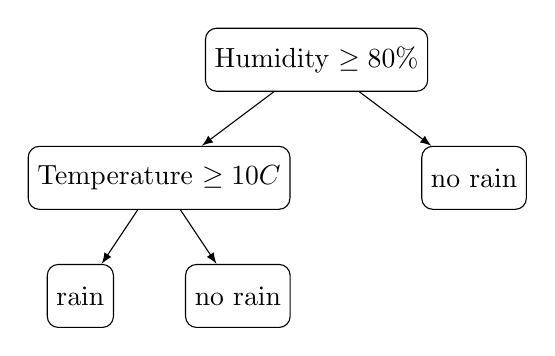
\begin{tikzpicture}[
			% Define styles for nodes
			level 1/.style={sibling distance=40mm},
			level 2/.style={sibling distance=20mm},
			level 3/.style={sibling distance=10mm},
			every node/.style={draw, rectangle, rounded corners, align=center, minimum size=8mm},
			edge from parent/.style={draw, -latex}
		]

		% Root node
		\node {Humidity $\geq 80\%$}
		% First level
		child {node {Temperature $\geq 10C$}
				% Second level
				child {node {rain}}
				child {node {no rain}}
			}
		child {node {no rain}};
	\end{tikzpicture}
	\caption{A very simple example of decision tree built on the mock problem}
	\label{fig:simple-dt}
\end{figure}
\subsection{Indices and node split computation}
In \cref{fig:simple-dt} a simple structure for a decision tree was shown, an excellent question in
its regard could be: 'Why this structure and not another?'. Other than it being a simple example
nothing is really preventing us from describing the 'rain' event based on different threshold values
or different feature sets altogether.
\begin{figure}
	\centering
	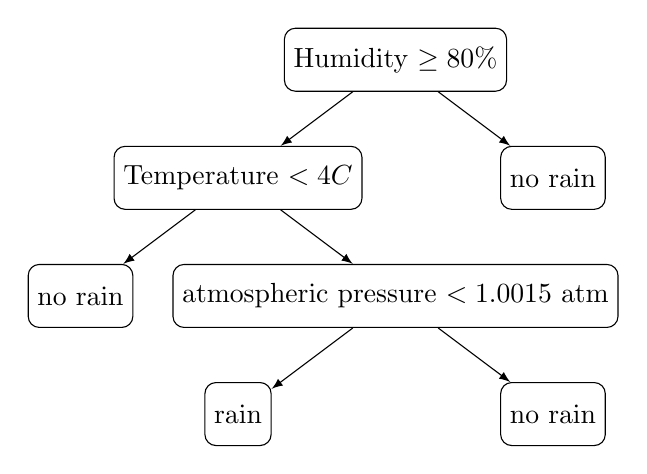
\begin{tikzpicture}[
			% Define styles for nodes
			level 1/.style={sibling distance=40mm},
			level 2/.style={sibling distance=40mm},
			level 3/.style={sibling distance=40mm},
			every node/.style={draw, rectangle, rounded corners, align=center, minimum size=8mm},
			edge from parent/.style={draw, -latex}
		]

		% Root node
		\node {Humidity $\geq 80\%$}
		% First level
		child {node {Temperature $< 4C$}
				% Second level
				child {node {no rain}}
				child {node {atmospheric pressure $< 1.0015$ atm}
						child{node {rain}}
						child{node {no rain}}
					}
			}
		child {node {no rain}};
	\end{tikzpicture}
	\caption{A very simple example of decision tree built on the mock problem}
	\label{fig:simple-dt-alt}
\end{figure}
The mock tree shown in \cref{fig:simple-dt-alt} is a different tree compared to the one shown in
\cref{fig:simple-dt} and yet they solve the same problem by characterizing it differently.
\cref{algo:decision-tree} shows how the decision tree is built, line $9$ states that the best
splitting feature needs to be selected with every iteration, this choice is taken based on a
\emph{purity} index applied to nodes.

\begin{algorithm}
	\caption{The decision tree base algorithm taken from
		\cite{ZhouZhi-Hua2021ML}}\label{algo:decision-tree}
	\begin{algorithmic}[1]
		\Require Training set $\dset$ and Feature set $A = \{a_1, \ldots,
			a_d\}$.
		\Ensure A decision tree with root node $i$
		\Function{TreeGenerate}{$D$, $A$}
		\State Generate node $i$;
		\If{All samples in $D$ belong to the same class $C$}
		\State Mark node $i$ as a class $C$ leaf node; \textbf{return}
		\EndIf
		\If{$A = \emptyset$ \textsc{or} all samples in $D$ take the same
			value on $A$}
		\State Mark node $i$ as a leaf node, its class label is
		the majority in $D$; \textbf{return}
		\EndIf
		\State Select the optimal splitting feature $a_*$ from $A$;
		\For{each value $a_*^v$ on $a_*$}
		\State Generate a branch for node $i$; Let $D_v$ be the
		subset of samples taking value $a_*^v$ on $a_*$;
		\If{$D_v$ is empty}
		\State Mark this child node as a leaf node, and
		label t with the majority class of $D$;
		\textbf{return}
		\Else
		\State use \textproc{TreeGenerate}$(D_v, A \setminus \{a_*\})$ as the child node.
		\EndIf
		\EndFor
		\EndFunction
	\end{algorithmic}
\end{algorithm}

\medskip

The purity of a node defines how many samples belong to a single class \cite{ZhouZhi-Hua2021ML}, a
split is going to be performed on feature $a$ only if the resulting purity increase is the best
possible. There are many different indices used to compute purity, in the following I will be
considering only the ones important for the model selection process that will be introduced in
a future chapter: \emph{Entropy} and \emph{Gini index}.

\subsubsection{Entropy}
There are many different ways of defining information entropy, a more general definition, compared
to the one found in \cite{ZhouZhi-Hua2021ML}, is found in \cite{gray2011entropy}. Let's consider a
random variable $f$ built on the alphabet $B = \{b_1, \ldots, b_{|B|}\}$ we can define the
partition $\mathcal{Q} = \{Q_i: i = 1, \ldots, |B|\}$ where $Q_i = \{\omega: f(\omega) = b_i\} = f^{-1}(b_i)$ therefore $\mathcal{Q}$ is a partition of the bigger
probability space $\Omega$, every partition is chosen based on the outcome of the
measurement of the random variable $f$. In the case of a discrete random variable we can define the
information entropy as shown in \cref{eq:information-entropy}
\begin{equation}
	\label{eq:information-entropy}
	H_p(\mathcal{Q}) = - \sum_{i = 1}^{|B|}{P(Q_i)\log{P(Q_i)}}
\end{equation}
this definition of entropy can be easily extended to the dataset case since:
\begin{itemize}
	\item The partition set $\mathcal{Q}$ can be mapped to the dataset $D$,
	\item Every partition $Q_i$ can be mapped to the single class of the machine learning
	      problem that is being considered,
	\item The alphabet $B$ can be mapped to the set of possible outcomes of the machine learning
	      problem.
\end{itemize}
Therefore, we can rewrite \cref{eq:information-entropy} as:
\begin{equation}
	H_p(D) = - \sum_{k = 1}^{|\outs|}p_k \log{p_k}
\end{equation}
$p_k$ denotes the proportion of the $k$-th class inside dataset $D$.

If we consider the binary classification problem ('true' or 'false' response), whenever a splitting procedure
is done on a node in the tree, the split is computed on every feature based on the possible
values of the feature itself (only for discrete features), if we consider our mock-problem, a split could be computed on a
feature called  'status of the sky' which can have one of two values $\{\text{overcast},
	\text{clear}\}$ the new node could be built in two different ways and
the class distribution for each is different, having different levels of purity based
on how well the data is partitioned between the classes 'rain' and 'no rain'.

\smallskip

To choose which of the two nodes to take in our mock-problem using the entropy measure we need to
introduce the concept of \emph{information gain}, which is expressed as follows:
\begin{equation}
	\label{eq:information-gain}
	\textsc{Gain}(D, a) = H_p(D) - \sum_{v = 1}^V\frac{|D^v|}{|D|}H_p(D^v)
\end{equation}
The concept expressed by information gain in \cref{eq:information-gain} is that the amount of
information gained by doing a split of dataset $D$ on feature $a$ is given by the entropy of dataset
$D$ at the moment of the split from which we remove the entropy of the dataset resulting from the
split of feature $a$ at every value $v$ scaled by the ratio between the cardinality of the new dataset to
the cardinality of the original dataset.

\smallskip

The feature used to perform the actual splitting is going to be the one with the highest possible
information gain. It's very important to notice that information gain is an index biased towards
features that have many different values (and therefore $|D^v|$ is small). In the case of our mock
problem, if we consider 'status of the sky' and we compare it to another feature containing many
different splitting values for example 'cloud color' which might assume the following values
$\{\text{white}, \text{light grey}, \text{grey}, \text{black}, \text{pink}, \text{orange},
	\text{red}\}$ it's clear that the $|D^v|/|D|$ is going to be lower for each of them, therefore
leading to a lower entropy decrease and a higher information gain.

\medskip

The alternative to using information gain is to use the \emph{gain ratio}
\begin{equation}
	\label{eq:gain-ratio}
	\textsc{GainRatio}(D, a) = \frac{\textsc{Gain}(D, a)}{\textsc{iv}(a)}
\end{equation}
the \textsc{iv} function in \cref{eq:gain-ratio} is the \emph{intrinsic value} of feature $a$ and
can be computed as shown in \cref{eq:intrinsic-value}.
\begin{equation}
	\label{eq:intrinsic-value}
	\textsc{iv}(a) = - \sum_{v = 1}^V\frac{|D^v|}{|D|} \log{\frac{|D^v|}{|D|}}
\end{equation}
Due to how intrinsic value is defined the gain ratio corrects the bias of the information gain towards features
with a higher number of values but is biased towards features with a lower amount of variables
\cite{ZhouZhi-Hua2021ML}.

In the actual implementation of the decision tree provided by scikit-learn an optimized version of
the \textsc{cart} algorithm is used, which  is similar to the \textsc{c4.5} algorithm proposed by Quinlan in
\cite{quinlan2014c4}.

\subsubsection{Gini index}
The original \textsc{cart} algorithm conceptualized by Breiman et al. in 1984
\cite{breiman1984classification} used Gini index to compute the best splitting feature for every
node. The Gini value of a dataset can be computed as shown in \cref{eq:gini-value}
\begin{equation}
	\label{eq:gini-value}
	\textsc{Gini}(D) = \sum_{k = 1}^{|\outs|}\sum_{k' \neq k} p_kp_{k'} = 1 - \sum_{k =
		1}^{|\outs|}p_k^2
\end{equation}
As explained in \cite{ZhouZhi-Hua2021ML}, \cref{eq:gini-value} can be interpreted as the
likelihood of taking samples from two different classes by drawing them randomly from the
dataset, the lower the $\textsc{Gini}(D)$, the higher the purity of a node. Gini index can be
computed as the weighted sum of all the Gini values for the dataset after the split, as shown in
\cref{eq:gini-index}.
\begin{equation}
	\label{eq:gini-index}
	\textsc{GiniIdx}(D) = \sum_{v = 1}^V\frac{|D^v|}{|D|} \textsc{Gini}(D^v)
\end{equation}

The best splitting feature is going to be the one with the smallest Gini index overall.

\subsection{Avoiding overfitting through pre- and post- pruning}
As was argued in the previous section decision trees have an extremely simple structure and they
allow us to interpret the obtained results giving us an idea of how the machine is able to classify
our points.

Overfitting is probably the biggest drawback of decision trees, as shown in
\cite{overfitting-dt-erblin}, since the model tries to partition the space based on the purity of
the nodes it's important to make sure that the rules utilized to do partitioning do not become too
specific. There are two techniques explained in the literature that can be used to prevent the model
from overfitting: Pre-pruning and post-pruning.

\medskip

Pre-pruning consists in a set of rules that force the algorithm to an early stop whenever a series
of conditions allow it. In the literature pre-pruning is sometimes associated only to a technique
that stops the splitting procedure whenever the impurity decrease (or the purity increase) doesn't
justify the split in the first place \cite{ZhouZhi-Hua2021ML}; I find myself more in line with
the general definitions given in \cite{bramer2007principles}\cite{fisher1996learning}, which
state that pre-pruning is a group of techniques meant to keep the size of the tree in check.

The specific pre-pruning conditions that can be checked using the DecisionTreeClassifier class provided by
scikit-learn are the following:
\begin{itemize}
	\item The tree \emph{depth}, avoiding a complex tree structure by cutting the depth is
	      probably one of the easiest forms of pre-pruning.
	\item The \emph{impurity decrease} stops nodes from splitting when the decrease in impurity
	      of the children is not higher than a certain threshold, if the threshold is too high
	      then the tree will probably underperform, if it's too low then the tree is going to
	      overfit.
	\item The \emph{number of elements to split} is basically a check that can be done on the
	      number of points inside a node. Not splitting when the number of points
	      contained in a node is too little is ax excellent way of avoiding overfitting.
\end{itemize}

\medskip

Post-pruning is the alternative to pre-pruning, the essential difference between the two is that
post-pruning is done after the tree has been fully constructed, therefore, in the a posteriori phase
a series of branches will be chosen to be pruned based on the impurity decrease that they provide.
There are different post-pruning techniques that can be implemented, scikit-learn is working with
Cost Complexity Pruning (\textsc{ccp}), introduced in \cite{breiman1984classification}.

\section{Random Forests}
\label{sec:rf}
The second model that I used in the project is the \emph{RandomForestClassifier} part of the scikit-learn
library. Random Forests are an \emph{ensemble} of trees, if different models are put together to solve a
problem, the performance will surely be higher than using a single tree, this is especially true for
weaker models, the reason why we chose to explore random forests is because the model is expected to
perform better than single trees, especially in the case of weaker datasets (such as Bn, results
will be introduced in a later chapter).

\medskip

Following the analysis done in \cite{ZhouZhi-Hua2021ML}, I will now prove that the error rate of a
binary classifier based on an ensemble of models grows to zero based on the number of individuals
used.

Let's suppose that the error rate of each model in the ensemble is $\epsilon$, the ground truth
function is $f$ and the single learner is $l_i$, then we can express the probability of the learner
making a wrong prediction on $\vec{x} \in \ins$ as shown in \cref{eq:error-rate}.
\begin{equation}
	\label{eq:error-rate}
	P(l_i(\vec{x}) \neq f(\vec{x})) = \epsilon
\end{equation}
Assuming that the prediction is $y \in \{-1, +1\}$ and the ensemble aggregates the predictions by
using a simple majority algorithm, then the aggregated prediction can be described as shown in
\cref{eq:ensemble-aggregation}.
\begin{equation}
	\label{eq:ensemble-aggregation}
	F(\vec{x}) = sign\left(\sum_{i = 1}^{T}l_i(\vec{x})\right)
\end{equation}
The probability of the ensemble being wrong is equal to computing the probability that more than
half of the single learners are independently wrong. The number of estimators being wrong in the
ensemble can be expressed as a binomial random variable $X \sim B(T, \epsilon)$. Therefore, we can finish our proof as shown in \cref{eq:binomial} and \cref{eq:hoeffding}
\begin{equation}
	\label{eq:binomial}
	P(F(\vec{x}) \neq f(\vec{x})) = P(X > T / 2) = \sum_{k = 0}^{\lfloor T / 2 \rfloor}\binom{T}{k} (1 -
	\epsilon)^k\epsilon^{T - k}
\end{equation}
Then for the Chernoff-Hoeffding inequality we can conclude that the error rate of the ensemble falls
exponentially with the number of estimators.
\begin{equation}
	\label{eq:hoeffding}
	\sum_{k = 0}^{\lfloor T / 2 \rfloor}\binom{T}{k} (1 - \epsilon)^k\epsilon^{T - k} \leq
	exp\left(-\frac{1}{2}T(1 - 2\epsilon)^2\right)
\end{equation}
\comment{Make sure that the proof is correct}{There are a series of things that I have said in the
proof that do not quite convince me}

Random forests work on a subset of features of size $k$ picked randomly from the set of features,
the size of the subset determines the behavior of the model, the splitting procedure works in the
same way exposed in \cref{sec:dt} if $k = d$, if $k = 1$, the split will be operated on a random
feature every time. In scikit-learn random forests are built out of trees that are constructed by
bootstrap sampling, a new dataset is built by doing a repeated draws without deletion from the
original dataset. The splitting process will be operated either by computing checking the whole
feature set or by checking a random subset of the feature set which size is regulated by one of the
attributes of the object.

\comment{Think about something else to write}{The section feels empty compared to the one about
decision trees}

\section{SVM}
\label{sec:svm}
With this section we leave behind the tree-based models to talk about the benchmark model that we
chose for this thesis, an \svm is a model with very high performance but low explainability, in this
chapter I will give some theoretical context to the model. Most of what will be said in this section
was taken from the main reference for the machine learning chapter \cite{ZhouZhi-Hua2021ML}.

\medskip

Let's consider a binary classification problem on dataset $\dset$ with labels $y \in \{-1, +1\}$,
handling the classification task means to find a hyperplane that is able to divide the points in the
dataset 'reasonably well', since the number of such hyperplanes is infinite there are two
essential observations to be made:
\begin{enumerate}
	\item The space of the solutions cannot be checked thoroughly, therefore we will never know
	      if the hyperplane chosen is the best one or if there is another that yields better
	      performance.
	\item The hyperplane that we are choosing will be fitted on the dataset used for training,
	      but we can make sure that the generalization performance are good enough by making
	      sure that there is enough \emph{margin} between the separator and the 'hardest'
	      points contained within the dataset.
\end{enumerate}
The hardest points are the ones closest to the hyperplane and they are called \emph{support
	vectors}.

\medskip

We can express any hyperplane in space as a function (\cref{eq:hyperplane}) of a vector $\vec{w}$ which is a normal vector
controlling the direction of the hyperplane and a bias $b$ value which controls the distance from
the origin.
\begin{equation}
	\label{eq:hyperplane}
	\vec{w}^\top\vec{x} + b = 0
\end{equation}
For any given point in space we can compute its distance from the hyperplane as shown in
\cref{eq:hyperdistance}.
\begin{equation}
	\label{eq:hyperdistance}
	r = \frac{|\vec{w}^\top\vec{x} + b|}{||\vec{w}||}
\end{equation}
Let's suppose that the hyperplane can perfectly divide the points in the two classes, we can
describe it as shown in \cref{eq:system}.
\begin{equation}
	\label{eq:system}
	\begin{cases}
		 & \vec{w}^\top\vec{x}_i + b > 0, \hspace{10pt} y_i = +1 \\
		 & \vec{w}^\top\vec{x}_i + b < 0, \hspace{10pt} y_i = -1
	\end{cases}
\end{equation}
\Cref{eq:svm-system} is valid for every point in the dataset, but we can give a stronger condition
which only works for the support vectors and is based on the distance defined in
\cref{eq:hyperdistance}. This new system is shown in \cref{eq:svm-system}.
\begin{equation}
	\label{eq:svm-system}
	\begin{cases}
		 & \vec{w}^\top\vec{x}_i + b \geq +1, \hspace{10pt} y_i = +1 \\
		 & \vec{w}^\top\vec{x}_i + b \leq -1, \hspace{10pt} y_i = -1
	\end{cases}
\end{equation}
The margin is the total distance between two support vectors belonging to different classes is
called margin and is defined in \cref{eq:margin}.
\begin{equation}
	\label{eq:margin}
	\gamma = \frac{2}{||\vec{w}||}
\end{equation}

\medskip

As was said in the beginning of this section we want to find the best separating hyperplane,
therefore the hyperplane that has a reasonable distance from the hardest points in the training set
to guarantee good generalization performance. We can express this problem as a maximization problem:
we want to maximize the margin in \cref{eq:margin} subject to the constraints of
\cref{eq:svm-system}. Maximizing the margin means maximizing $||\vec{w}||^{-1}$ which is equivalent
to minimizing $||\vec{w}||^2$, taken for simplicity purposes. The problem, as is formulated in
\cref{eq:primal}, is the primal form of \svm.
\begin{equation}
	\label{eq:primal}
	\begin{aligned}
		 & \max_{\vec{w}, b}\frac{1}{2}||\vec{w}||^2                                                   \\
		 & \text{s.t.}\hspace{10pt}y_i(\vec{w}^\top\vec{x}_i + b) \geq 1 \hspace{10pt}i = 1, \ldots, m
	\end{aligned}
\end{equation}
This is a quadratic programming problem, there are libraries that provide solvers for the problem,
but there are other methods that allow us to compute a solution with a higher grade of efficiency.
We can introduce \emph{Lagrange multipliers} and the \emph{lagrangian} can be expressed as shown in
\cref{eq:lagrangian}.
\begin{equation}
	\label{eq:lagrangian}
	\lag(\vec{w}, b, \vec{\alpha}) = \frac{1}{2} ||\vec{w}||^2 + \sum_{i = 1}^{m}{\alpha_i (1 - y_i(\vec{w}^\top\vec{x}_i + b))}
\end{equation}
If we compute the partial derivatives of the lagrangian with respect to $\vec{w}$ and the bias $b$
we obtain the two equations shown in \cref{eq:pd-lagrangian}.
\begin{equation}
	\label{eq:pd-lagrangian}
	\begin{aligned}
		 & \frac{\partial{\lag}}{\partial{\vec{w}}} = \vec{w} - \sum_{i = 1}^m
		\alpha_iy_i\vec{x}_i                                                   \\
		 & \frac{\partial{\lag}}{\partial{b}} = \sum_{i = 1}^m \alpha_iy_i
	\end{aligned}
\end{equation}
By setting the partial derivatives just shown to zero and substituting the first in
\cref{eq:lagrangian} we can get rid of the normal vector dependency and the \emph{dual} problem can
be defined as a function of $\vec{\alpha}$ and the bias $b$. The dual problem is shown in \cref{eq:dual}.
\begin{equation}
	\label{eq:dual}
	\begin{aligned}
		 & \max_{\vec{\alpha}}\left(\sum_{i = 1}^{m}{\alpha_i} - \frac{1}{2}\sum_{i =
		1}^{m}\sum_{j = 1}^{m}{\alpha_i\alpha_j y_i y_j \vec{x}_i\vec{x}_j}\right)       \\
		 & \text{s.t.} \sum_{i = 1}^{m}{\alpha_i y_i} = 0 \hspace{10pt} i = 1, \ldots, m
	\end{aligned}
\end{equation}
The hyperplane that we are looking for can be modelled as shon in \cref{eq:of}, the second
formulation is virtue of the substitution found for $\vec{w}$ in \cref{eq:pd-lagrangian}.
\begin{equation}
	\label{eq:of}
	f(\vec{x}) = \vec{w}^\top\vec{x} + b = \sum_{i = 1}^m\alpha_iy_i\vec{x}_i\vec{x} + b
\end{equation}
Since the primal problem \cref{eq:primal} is an optimization problem with inequality constraints we
know from \cite{kkt1951} that solving it is equivalent to solving the dual problem based on the
lagrangian defined in \cref{eq:lagrangian} subject to the \textsc{kkt} constraints shown in
\cref{eq:kkt-constraints}.
\begin{equation}
	\label{eq:kkt-constraints}
	\begin{cases}
		 & \alpha_i \geq 0                   \\
		 & y_if(\vec{x}_i) - 1 \geq 0        \\
		 & \alpha_i(y_if(\vec{x}_i) - 1) = 0
	\end{cases}
\end{equation}
For every point in the training set $(\vec{x}_i, y_i)$ only two scenarios are possible:
\begin{enumerate}
	\item Lagrange multiplier $\alpha_i = 0$, therefore the point is not impacting the
	      hyperplane structure as was defined in \cref{eq:of}.
	\item If the Lagrange multiplier $\alpha_i > 0$ then the third constraint in
	      \cref{eq:kkt-constraints} yields $y_if(\vec{x}_i) = 1$ which means that the point is
	      laying on the maximum margin hyperplanes, therefore it's a support vector.
\end{enumerate}
This reveals a very important detail: once the training is completed, the model can be entirely
described by using only support vectors, since they are the ones that yield a contribution in the
calculation of \cref{eq:of}.

There are different techniques to solve \cref{eq:dual} one of the possibilities is to use quadratic
programming solvers, another possibility is to use the \textsc{smo} method proposed in
\cite{platt1998} and consisting in an iterative resolution of the problem by successive
identifications of local approximations of the Lagrange multipliers $\alpha_i$ while keeping all
other parameters frozen as constants.

\medskip

The method exposed in this section provides a solution to problem \cref{eq:primal} which is meant to
have perfect accuracy, meaning that no classification errors are acceptable. This is a solution that
is neither advisable nor possible in most cases due to the problem of linear separability addressed
in \cref{sssec:kernel-functions}.

For this reason the \emph{soft margin} \svm model was defined, such formulation of the solution
allows a relaxation of the constraints and therefore a certain number of classification errors.
Since the number of errors needs to be minimized we can rewrite the objective of \cref{eq:primal} as
shown in \cref{eq:sm-primal}.
\begin{equation}
	\label{eq:sm-primal}
	\min_{\vec{w}, b} \frac{1}{2}||\vec{w}||^2 + C\sum_{i = 1}^m \ell_{0 / 1}(y_i (\vec{w}^\top \vec{x}_i + b) - 1)
\end{equation}
In equation \cref{eq:sm-primal} $C > 0$ is a regularization constant, $\ell_{0 / 1}$ is the $0/1$
loss; solving directly the equation can be really complex due to the poor mathematical properties of
the $0/1$ loss function properties and, even though there are approximate methods to minimize the
function \cite{nguyen2013}, most of the time a convex loss function is used to replace the $0/1$
loss.

Soft margin \svm is defined by substituting $0/1$ loss with hinge loss and then adding slack
variables $\psi_i \geq 0$ the primal problem can be easily rewritten as shown in
\cref{eq:sm-primal-final}.
\begin{equation}
	\label{eq:sm-primal_final}
	\min_{\vec{w}, b} \frac{1}{2}||\vec{w}||^2 + C\sum_{i = 1}^m \psi_i
\end{equation}


In the following I am going to remove a big assumption that was silently made in the beginning and I
will provide some adjustments to the model.

\subsubsection{Kernel funtions}
\label{sssec:kernel-functions}
Until now the topic was treated under the important assumption that the points in the dataset are
linearly separable, but it's known that commonly this condition doesn't hold, since most problems
treated in the real world are not linearly separable. To address the issue the
problem is moved to a higher dimensionality space through a mapping $\phi(\cdot)$. We know from
Cover's theorem \cite{cover1965} that if the number of features is finite then there must be a
projection to a high dimensionality space that provides linear separability for the data.

If we define $\phi(\vec{x})$ the mapping of a data-point $\vec{x} \in \ins$ to the high
dimensionality space we can rewrite \cref{eq:hyperplane} to incorporate this mapping.
\begin{equation}
	\label{ep:hd-hyperplane}
	f(\vec{x}) = \vec{w}^\top \phi(\vec{x}) + b
\end{equation}
Using \cref{ep:hd-hyperplane} and following the reasoning shown in the beginning of the section,
it's possible to redefine both the primal (\cref{eq:primal}) and the dual (\cref{eq:dual}) problems
as shown in \cref{eq:hd-primal} and \cref{eq:hd-dual}
\begin{equation}
	\label{eq:hd-primal}
	\begin{aligned}
		 & \max_{\vec{w}, b}\frac{1}{2}||\vec{w}||^2                                                   \\
		 & \text{s.t.}\hspace{10pt}y_i(\vec{w}^\top\phi(\vec{x}_i) + b) \geq 1 \hspace{10pt}i = 1, \ldots, m
	\end{aligned}
\end{equation}
\begin{equation}
	\label{eq:hd-dual}
	\begin{aligned}
		 & \max_{\vec{\alpha}}\left(\sum_{i = 1}^{m}{\alpha_i} - \frac{1}{2}\sum_{i =
		1}^{m}\sum_{j = 1}^{m}{\alpha_i\alpha_j y_i y_j \phi(\vec{x}_i)^\top\phi(\vec{x}_j})\right)       \\
		 & \text{s.t.} \sum_{i = 1}^{m}{\alpha_i y_i} = 0 \hspace{10pt} i = 1, \ldots, m
	\end{aligned}
\end{equation}

As was done in the beginning of the section it would now be necessary to compute a solution of the
dual problem, which means computing the internal product $\langle\phi(\vec{x}_i),
\phi(\vec{x}_j)\rangle$, since the problem was moved to a high dimensional space it might be
computationally expensive to handle, especially because the number of dimensions of the final space
is not known.

To avoid having to compute such a product we define a function, known as \emph{kernel} function
$\kappa(\cdot, \cdot)$,
which is an approximation of the actual value of the inner product computed by using a function in
the input space. We can rewrite \cref{eq:hd-dual} to use the newly introduced function.
\begin{equation}
	\label{eq:hd-dual-kf}
	\begin{aligned}
		&\text{since} \hspace{10pt} \kappa(\vec{x}_i, \vec{x}_j) = \langle\phi(\vec{x}_i),
\phi(\vec{x}_j)\rangle \\
		 & \max_{\vec{\alpha}}\left(\sum_{i = 1}^{m}{\alpha_i} - \frac{1}{2}\sum_{i =
		1}^{m}\sum_{j = 1}^{m}{\alpha_i\alpha_j y_i y_j \phi(\vec{x}_i)^\top\phi(\vec{x}_j})\right)       \\
		 & \text{s.t.} \sum_{i = 1}^{m}{\alpha_i y_i} = 0 \hspace{10pt} i = 1, \ldots, m
	\end{aligned}
\end{equation}

If we solve the problem using the same procedure applied in the beginning of the section we obtain
an expression of the hyperplane which is dependent from the kernel function $\kappa$.
\begin{equation}
	\label{eq:hd-of}
	f(\vec{x}) = \sum_{i = 1}^m\alpha_iy_i\kappa(\vec{x}, \vec{x}) + b
\end{equation}

The kernel function was introduced earlier but no definition was given for it, since it depends on
the structure of the mapping $\phi$. Such mapping is unknown in most practical cases, however a
theorem grants us that if we can find a symmetric function $\kappa(\cdot, \cdot): \ins \rightarrow
\ins$, then $\kappa$ is going to be a kernel function if and only if, however chosen the dataset $D
= \{\vec{x}_1, \ldots, \vec{x}_m\}$, the kernel matrix $\mathbf{K}$ is going to be positive
semidefinite. Matrix $\mathbf{K}$ is constructed as shown in \cref{eq:kernel-matrix}.
\begin{equation}
	\label{eq:kernel-matrix}
	\mathbf{K} = 
	\begin{bmatrix}
		\kappa(\vec{x}_1, \vec{x}_1) & \kappa(\vec{x}_1, \vec{x}_2) & \ldots &
		\kappa(\vec{x}_1, \vec{x}_m) \\
		\kappa(\vec{x}_2, \vec{x}_1) & \kappa(\vec{x}_2, \vec{x}_2) & \ldots &
		\kappa(\vec{x}_2, \vec{x}_m) \\
		\ldots & \ldots & \ddots & \ldots \\
		\kappa(\vec{x}_m, \vec{x}_1) & \kappa(\vec{x}_m, \vec{x}_2) & \ldots &
		\kappa(\vec{x}_m, \vec{x}_m) \\
	\end{bmatrix}
\end{equation}
Now that a reliable technique to find kernel functions has been defined it's important to find the
best kernel function to the problem, since the choice of the kernel determines how the points are
mapped in high-dimensional space and therefore how good of a hyperplane is found.

\section{Unsupervised models}
\label{sec:uml}

\section{Clustering with k\-means}
\label{sec:kmeans}

\chapter{The problem}
\label{chp:problem}
Following~\cite{mariotto2022}, the HO corrector magnets have been designed to produce five different multipolar field orders (quadrupole, sextupole, octapole, decapole, and dodecapole). Tested at cryogenic temperature, the magnets are powered to evaluate their performances and thermal stability up to the nominal operating condition. During magnet powering, spontaneous quench transitions in the superconducting coil volume can occur due to mechanical instability of the winding or stress induced by the electromagnetic Lorentz forces acting on the conductors. Each magnet is protected using a classical resistive voltage detection system and discharged on an external dumping resistance to extract most of the stored magnetic energy from the magnet to prevent any material damage. Limited to analyzing only two separate voltage signals connected in parallel to the coils, the quench detection system can only evaluate if a quench development occurred in half of the magnet coils without the possibility to localize precisely which superconducting winding started the transition to the normal conducting state. To retrieve this information and evaluate if a possible degradation of the coil has occurred, a magnetic field measurement-based model has been proposed analyzing the residual magnetic field quality produced by the non-quenched superconducting coils in the magnet after the quench event. The original work proposed a study specific to quadrupoles, since they gave the majority of the positives (quench events), which have been used as the subject of this analysis, therefore ignoring all other configurations focusing only on the five quadrupoles of the series production from MQSXF1 to MQSXF6.
\begin{figure}[h!]
	\centering
	\includegraphics[width=\linewidth]{img/FieldProcedure.pdf}
	\caption{Sketch of the magnetic field measurements after a quench event for the quadrupole magnet and dataset obtained for each quench event measurement.}
	\label{fig:FieldMeasurement}
\end{figure}
As a result of the magnets test campaign, $279$ events, after the magnet discharge (quench event) or equivalent at zero operating current (non-quench event), were analyzed sampling the magnetic field in the magnet bore volume using a magnetic field rotating shaft.

For each event, 60 samples of measured harmonic coefficients have been measured and averaged to obtain a single set of $15$ different magnetic field harmonics coefficients which contain all the information of the produced magnetic field quality (see Fig.~\ref{fig:FieldMeasurement}). Recalling that these coefficients are expressed as complex numbers, the information have been organized in terms of the following four attributes, in which the suffix $n \in \{1, \dots,  15\}$ is related to a specific harmonic:
\begin{itemize}
	\item the imaginary part \an, of the $n^\text{th}$ field harmonic coefficient;
	\item the real part \bn, of the $n^\text{th}$ field harmonic coefficient;
	\item the absolute value \cnmod, of the $n^\text{th}$ field harmonic coefficient;
	\item the phase \phin, of the $n^\text{th}$ field harmonic coefficient.
\end{itemize}
In the experiment generating data, the magnets were mounted skewed: as a consequence, the $A_n$ feature was supposed to be highly informative since they are directly correlated with the rotational position of the quenched coil in the magnet assembly. The absolute values $|C_n|$ would be a valuable feature for \qrp{} and not for \qlp{} since two different configurations with the same number of quenched coils but different angular positions would give the same harmonic content and different phases. Each measurement was coupled with a \emph{label} encoded as follows:
\begin{itemize}
	\item a simple binary flag for \qrp, where $1$ means that a quench has happened, while $0$ characterizes the normal working conditions of the superconductor;
	\item four binary flags for \qlp, each describing a  coil and stating whether or not a quench happened within it, using the same encoding as in previous point.
\end{itemize}

In the following chapters we will not be using attributes in their entirety, in most cases the
datasets will be aggregating the best harmonics for a certain attribute (e.g., harmonics $2$ and
$12$ for attribute \an). We will be referring to these as sub-views of an attribute.

The objective of the thesis was to find machine learning models capable of:
\begin{enumerate}
	\item Recognizing whether the magnet underwent a quench event during operation, we will refer
	      to it as Quench Recognition Problem (\qrp) from now on, and will be treated in
	      \Cref{chp:qrp},
	\item Recognize, if the superconductor quenched, which coil(s) transitioned; we will refer to
	      it as Quench Localization Problem (\qlp) from now on, and it will be treated in
	      \Cref{chp:qlp}.
\end{enumerate}
The models chosen to solve \qrp\ and \qlp\ had to be both reliable and highly explainable to favour
further study of quench phenomenon on High-Order corrector magnets.

\section{Model selection and model testing procedures}
Reproducibility is a key property of any experiment, to cover the basics, we set the seed for all
random number generators to the same value, and we used shared pipelines for all our experiments.

Sub-views are built using a common pipeline that generates three different datasets, serialized
for later reuse:
\begin{itemize}
	\item The \emph{merged} dataset, \dm, which constructs a single table out of all the
	      measurements done on the attribute(s) for the different magnets. Before serialization, the
	      data is standardized using an instance of the StandardScaler class, contained in
	      scikit-learn, trained on the dataset just created (minus the label column(s)).
	\item The \emph{blind-test} dataset, \db, contains a small part of the overall data available to us
	      ($29$ samples), these samples were kept locked until the experiments were considered
	      complete. Using the blind-test set we performed a final test on the models to see
	      how well the performance generalize on unseen data.
	\item The \emph{reduced} dataset, \dr, contains the rest of the samples, $250$ in total,
	      and is the main set used to perform experiments.
\end{itemize}

Model selection and testing were carried out using Nested Cross Validation (\ncv). \ncv\ is suitable
for situations in which the data is not abundant~\cite{Larracy2021} due to its heavy reuse, enabling
model selection and testing, while also giving less biased performance estimates by averaging the
results on $k$ different folds, in the following section we will do a rapid excursus on how the
cross-validation procedure works.

\subsubsection{Cross Validation}
In \Cref{chp:ml} we talked about the simple train-test splitting procedure, now we will introduce an
alternative technique for splitting that gives us a powerful tool to prevent overfitting and get
less biased performance measures while also doing hyperparameter selection.

In general, given a dataset $D$, $k$-fold \cv~\cite{ZhouZhi-Hua2021ML} is a technique for splitting
a dataset in $k$ different folds $\fold{i}, i \in \{1, \ldots, k\}$, the folds are non-overlapping
and about the same size, therefore $\fold{i} \cap \fold{j} = \emptyset \hspace{5pt} \forall i, j \in
	\{1, \ldots, k\}, i \neq j$, and the union of all the folds is the original dataset ($\bigcup_{i \in \{1, \ldots, k\}} \fold{i} = D$).

\medskip

In the framework of train-test splitting, if we used the procedure outlined in \Cref{chp:ml}, we
would split the original dataset into the training set $T$ and the generalization set $G$, train
$\model$ on $T$ and then test the performance on $G$. While this is a perfectly acceptable procedure
to gather performance metrics for a model it doesn't give us any certainty on how reliable the
obtained metrics actually are.


By measuring performance on different folds (each one is a training and testing procedure separate
from others), we get a more complete vision of the model performance, allowing us to recognize pathological
situations, like cases in which the standard deviation of the fold performance is very wide. To
understand how the folds are structured, let's consider an example in which $5$-fold \cv\ is
computed on a dataset containing $250$ samples: $5$ different models are generated, each time it
trained on $200$ samples and then tested on the remaining $50$ samples (the testing fold changes
with every iteration).

The number of folds to be used for \cv\ becomes another hyperparameter of the problem, since it
depends on many factors like the amount of available data or the required reliability of performance
reads. A large value of $k$ will increase the number of folds the model is trained and tested on,
increasing the robustness of the performance estimation at the expense of computational complexity
(e.g., Leave One Out \cv\ is an example of such approaches, in~\cite{shao2016} a more efficient
approach to the technique is discussed); too small a value of $k$ makes the \cv\ less robust but more efficient (classic values of $k$ for most practical uses are $5, 10, 20$).

\medskip

Let us now move to a more complicated environment in which we need, given a base model, to do model
selection, do model training and finally do model testing. We can na\"ively tripartition dataset $D$:
\begin{itemize}
	\item \emph{Training set} $T$,
	\item \emph{Validation set} $V$, this set of samples will be used to test the performance of the
	      model found after the training step,
	\item \emph{Generalization set} $G$, after the model is retrained on $T + V$ the performance are
	      tested on $G$ to see if the model is capable of generalizing effectively.
\end{itemize}

Once again we cannot guarantee that:
\begin{inparaenum}[(i)]
	\item the chosen model is the best one,
	\item the performance metrics obtained from the single generalization fold are actually reliable.
\end{inparaenum}
To address the issue we can substitute each procedure with $k$-fold \cv, one nested inside of each
other, the \emph{inner} is used to do model selection, the \emph{outer} is used to test performance
for the model just generated. To get a better understanding of the Nested cross-validation procedure
(\ncv) just introduced let us consider a $5 \times 5$ \ncv\ procedure applied to a dataset of $250$
samples(an outline of the \ncv\ procedure is shown in \Cref{fig:nested-cv}).
\begin{itemize}
	\item The data is first split into $5$ folds of $50$ samples. One fold of $50$ samples will
	      be kept on the side for the generalization test, the remaining $200$ samples will be used to do both training and model selection;
	\item The training set is now split again in $5$ folds, $160$ samples will be used to do
	      model selection (therefore hyperparameter space search), $40$ samples will be used
	      to validate the performance that has been found;
	\item The model found at the previous step is retrained on the whole $200$ training samples and then
	      the performance are tested on the fold that was kept aside in the first step.
\end{itemize}
\begin{figure}[!t]
	\centering
	\includegraphics[scale=.3]{./img/nested-cv.png}
	\caption{Visualization of the nested cross validation procedure taken from~\cite{lavasa2021}}
	\label{fig:nested-cv}
\end{figure}

Once the \ncv\ procedure terminates we will get $k$ different models, since the fine-tuned models
are statistically equivalent, we can choose which one to keep using the heuristic that fits our
objectives the best.

The closing section for this chapter will contain a summarization of the experimental setup.

\section{Experimental setup}
The project was developed using the latest version of the Python programming language (3.10.12 at the moment of writing), All experiments have been executed using Python 3.10.12 (the latest version at the time of writing), using the following libraries: scikit-learn (release 1.5.2) for data preprocessing and model training and evaluation, numpy (release 2.2.3) for efficient data storage, and Pandas (release 2.2.3) for data management. These libraries have been handled through the pip package manager (release 25.0.1) and used within a virtual environment.

\medskip

The seeds from the various random number generators have been set to the common value of
\href{https://www.google.com/search?q=the+answer+to+life+the+universe+and+everything&num=10&client=firefox-b-d&sca_esv=a81abf9bb67ffd9b&sxsrf=AHTn8zo6RKep_zuEvIhJb5nuAGh5xAERLg\%3A1739739141586&ei=BVCyZ_C9I9mLi-gP7e-B8Ac&oq=the+answer+to+&gs_lp=Egxnd3Mtd2l6LXNlcnAiDnRoZSBhbnN3ZXIgdG8gKgIIADIIEAAYgAQYywEyCBAAGIAEGMsBMgUQABiABDIIEAAYgAQYywEyCBAAGIAEGMsBMggQABiABBjLATIIEAAYgAQYywEyCBAAGIAEGMsBMggQABiABBjLATIIEAAYgAQYywFIjCJQqQlYiRlwA3gBkAEAmAFuoAHICaoBBDExLjO4AQPIAQD4AQGYAhGgAv0JwgIKEAAYsAMY1gQYR8ICChAjGIAEGCcYigXCAgsQABiABBixAxiDAcICCxAuGIAEGLEDGIMBwgIOEC4YgAQYsQMY0QMYxwHCAg4QLhiABBixAxiDARiKBcICERAuGIAEGLEDGNEDGIMBGMcBwgIMECMYgAQYExgnGIoFwgIEECMYJ8ICDRAuGIAEGEMY1AIYigXCAgoQABiABBhDGIoFwgIOEC4YgAQYxwEYjgUYrwHCAgoQLhiABBhDGIoFwgIIEC4YgAQYsQPCAggQABiABBixA8ICCxAuGIAEGLEDGNQCwgIFEC4YgATCAggQLhiABBjLAcICCxAuGIAEGNEDGMcBmAMAiAYBkAYIkgcEMTIuNaAHrboC&sclient=gws-wiz-serp}{42} to prevent too much deviation in the experiments.

\medskip

The original contained $279$ samples, for \qrp, each sample consisted of $15$ harmonics and a Label
stating whether the sample represents a quench event ($1$) or not ($0$), for \qlp, each sample had $4$ different
labels associated to it representing whether one of the coils ($0$ for East, then: North, West and
South) quenched ($1$) or not ($0$).

Every splitting operation was performed by stratifying on the labels, in the case of \qlp, if the
labels were more than one, we used a multi-class stratification technique, detailed in (\cite{skmlearn}).

\medskip

Experiments were conducted on three different computers running different architectures and
different operating systems, but the results did not change due to the standard-oriented approach,
\Cref{tbl:computers} for a summary of the computers we used.
\begin{table}[t]
	\caption{System configuration used for our experiments. Core count values are detailed as number
		of CPU cores and threads, while frequency is expressed in the base and boost specifications.
		Finally, the CPU cache size is shown for the L1, L2 and L3 levels, where
		available.}\label{tbl:computers}

	\bigskip

	\centering
	\setlength{\tabcolsep}{4pt}
	\begin{tabular}{lccc}
		\toprule
		                     & \textbf{Pigna}        & \textbf{Mattone}         & \textbf{Topone}    \\
		\midrule
		\textbf{Model}       & Macbook Pro           & Custom build             & Dell XPS 8700      \\
		\textbf{CPU}         & i$5$ $5287\textsc{u}$ & Ryzen 7 $3700\textsc{x}$ & i$7$ $4770$        \\
		\textbf{Core count}  & $2\cc / 2\tc$         & $8\cc / 16\tc$           & $4\cc / 8\tc$      \\
		\textbf{Launch Date} & Q$1$ 2015             & Q$2$ 2019                & Q$2$ 2013          \\
		\textbf{Frequency}   & $2.90 / 3.30$ \ghz    & $4.125 / 4.40$ \ghz      & $3.40 / 3.90$ \ghz \\
		\textbf{Cache}       & $3$ \mb               & $0.512 / 4 / 32$ \mb     & $8$ \mb            \\
		\textbf{TDP}         & $28$ \w               & $84$ \w                  & $65$ \w            \\
		\textbf{RAM}         & $8$ \gb               & $16$ \gb                 & $16$ \gb           \\
		\textbf{OS}          & Pop!\_OS $22.04$ LTS  & Pop!\_OS $22.04$ LTS     & Fedora $39$        \\
		\bottomrule
	\end{tabular}
\end{table}
Experiments were dispatched on different systems based on the expected computational load.

Model selection was handled by doing a partial exploration of the parameter space via a grid search algorithm (GridSearchCV in scikit-learn), for each model we
defined a custom parameter grid (shown in \Cref{tbl:params}).

\begin{table}[t]
	\caption{Hyperparameters which we have tuned during the model training phase.} \label{tbl:params}

	\bigskip

	\centering
	\setlength{\tabcolsep}{6pt}
	\begin{tabular}{llc}
		\toprule
		\textbf{Model}       & \textbf{Hyperparameter}                                           & \textbf{Values}                        \\
		\midrule
		\multirow{5}{*}{DT}  & impurity criterion                                                & gini, entropy, log loss                \\
		                     & max depth                                                         & $2, 3, 4, 5$                           \\
		                     & min impurity decrease                                             & $0.001, 0.01, 0.05$                    \\
		                     & max features                                                      & None, $0.5, 0.75$                      \\
		                     & min samples leaf                                                  & $5, 10, 20$                            \\
		\midrule
		\multirow{1}{*}{RF}  & n. of trees                                                       & $2, 3, 5, 10$                          \\
		                     & \multicolumn{2}{l}{$+$ the same hyperparameters and values of DT}                                          \\
		\midrule
		\multirow{5}{*}{SVC} & $C$                                                               & $0.1, 1, 10, 100, 1000$                \\
		                     & $\gamma$                                                          & scale, auto, $0.001, 0.01, 0.1, 1, 10$ \\
		                     & degree                                                            & $2, 3, 4, 5$                           \\
		                     & $c_0$                                                             & $0, 0.1, 0.5, 1$                       \\
		                     & kernel                                                            & linear, poly sigmoid, rbf              \\
		\bottomrule
	\end{tabular}
\end{table}

All of the models have been tested on a suite of scorers meant to give us a more complete
understanding of how well the model is performing, the metrics are explained here below and, as
usual, by positive (negative) sample we mean a sample having label $1$ ($0$), and by true (false)
positive we mean a correctly classified positive (negative) sample:
\begin{itemize}
	\item \emph{Accuracy} (Acc): fraction of correct predictions,
	\item \emph{Precision} (Prc): number of true positives over number of positive predictions,
	\item \emph{Recall} (Rec): number of true positives over number of positive items,
	\item \emph{F1 score} (F1): harmonic mean between Precision and Recall,
	\item \emph{Inverse recall} (Irec): number of true negatives over number of negative items,
	\item \emph{ROC AUC} (RAUC): area under the receiver operating characteristic curve.
\end{itemize}
The main metric of our suite is going to be accuracy.






\chapter{Quench Recognition Problem (QRP)}
\label{chp:qrp}
This chapter is dedicated to the solution of \qrp, which we introduced in \Cref{chp:problem}, in this chapter we will:
\begin{itemize}
	\item Give a rapid overview of the problem, analyzing the results obtained from
	      preprocessing,
	\item Talk about the models used, and the results obtained for each model,
	\item Select the 'best' possible model.
\end{itemize}

\section{Data preprocessing}
\label{sec:qrp-preprocessing}
Before working on the actual models we analyzed:
\begin{itemize}
	\item the cross-correlations between the harmonics, which aims to identify repeated
	      information within the dataset;
	\item the cross-correlation between the harmonics and the labels, which indicates how
	      well the harmonics of the dataset are capable of explaining the expected results;
	\item the box plot of the attributes, which is visualizes the variability of the harmonics,
	      giving us a powerful tool to understand which ones are more relevant to the
	      computation, and
	\item the distribution of data after dimensionality reduction via principal component
	      analysis (\pca), which is meant to give a good idea of how the data are distributed
	      and hints to which are the better attributes to solve the problem.
\end{itemize}
In the following, the vector containing the information about the correlation with the labels has
been plotted after a normalization step, which was done by training an instance of the MinMaxScaler
class from scikit-learn. While this procedure doesn't change the intensity of the correlation
between the harmonic and the label it makes the plots more readable and easier to interpret, the normalized samples are scaled using \Cref{eq:normalization} \cite{Nishok2024}.
\begin{equation}
	\label{eq:normalization}
	X_\text{scaled} = \frac{X - X_\text{min}}{X_\text{max} - X_\text{min}}
\end{equation}
Where $X$ is a sample in the vector that is being scaled.

We will be covering the results of preprocessing in four different sections, each dedicated to one
attribute.

\subsubsection{\an}
\Cref{fig:an-corr} among the harmonics. Independently of the sign, the matrix evidently contains a
pattern, hinting to the fact that many harmonics contain repeated information, (e.g., \an[1] provides
the same information as \an[3], \an[5], \an[7]), \ldots By analyzing the figure we can reach the
following conclusions:
\begin{itemize}
	\item Its strong geometry implies that doing feature extraction is going to be complex (as
	      we will see in the following sections it's basically a shared characteristic for
	      almost all the attributes), due to the necessity of finding a mix of harmonics that has a high correlation with the label, while having a low correlation among themselves.
	\item All the odd harmonics are strongly correlated with each other (with the sole exception
	      of \an[15]),
	\item \an[2] is strongly correlated with its odd multiples (i.e., \an[6], \an[10], \an[14]),
	\item \an[4] is strongly correlated with all its multiples (i.e., \an[8], \an[12]),
	\item \an[15] is the only one not correlated to any of the other harmonics.
\end{itemize}
\begin{figure}[!ht]
	\centering
	\includegraphics[width=\linewidth]{img/An_corr_matrix.png}
	\caption{The cross-correlation among the \an\ harmonics.} \label{fig:an-corr}
\end{figure}

If we consider \Cref{fig:an-lcorr}, and we pick the harmonics with the highest label correlation,
identified by a higher color intensity, we end up with the following set of features: \{\an[2],
\an[6], \an[10], \an[11], \an[12], \an[13], \an[14], \an[15]\}. This is interesting because:
\begin{enumerate}
	\item \an[2], as well as its odd multiples, can explain the results well, which is what we expect from the theory.
	\item High order harmonics are able to explain the results better than other harmonics,
	      which is not what we would have expected, since in the original analysis the value for the
	      labels was computed using primarily low-order harmonics\footnote{By low order
		      harmonics we intend the harmonics going from $1$ to $6$ circa}.
\end{enumerate}

\begin{figure}[!ht]
	\centering
	\includegraphics[width=\linewidth]{img/An_label_corr.png}
	\caption{Correlation between the harmonics and the labels for \an.} \label{fig:an-lcorr}
\end{figure}

The structure of the correlation matrix and the correlation between labels and harmonics leads us to
believe that a good-performing sub-view for \an\ should contain \an[2], or one of its high-order
odd multiples, as well as \an[15]\ and some other high-order harmonics like \an[11]\ or \an[13].

Lastly, we can visualize the distribution of samples in bidimensional space, achieved by using \pca\
dimensionality reduction.
\begin{figure}[!ht]
	\centering
	\includegraphics[width=\linewidth]{img/An_distribution.png}
	\caption{Data distribution for the \an\ table after applying \pca\ dimensionality
		reduction, moving from $15$-dimensional space to $2$-dimensional space-dimensional
		space. In the plot we highlight quench and non-quench events.} \label{fig:an-dist}
\end{figure}

As we will see in the following sections, the distribution shown in \Cref{fig:an-dist}, with its
clear-cut clusters characterized by a high level of purity, is the best distribution among the
alternatives. Having such a good distribution lead us to think that it might be the reason why
models built on \an\ and \cnmod\ (at least for \qrp) perform better than the ones built on \bn\ and
\phin.

\subsubsection{\bn}
We can use a similar procedure on the \bn\ attribute, which in most tests proved to be the
least-performing attribute. This is probably due to the poor distribution of the data, as we can see in
\Cref{fig:bn-dist}, the central cluster has a very high level of homogeneity.
\begin{figure}[!ht]
	\centering
	\includegraphics[width=\linewidth]{img/Bn_distribution.png}
	\caption{Data distribution for the \bn\ table after applying \pca\ dimensionality
		reduction, moving from $15$-dimensional space to $2$-dimensional space-dimensional
		space. In the plot we highlight quench and non-quench events.} \label{fig:bn-dist}
\end{figure}

As we did for \an\ we checked the correlation among harmonics for the \bn\ attribute, the results
were very similar, the more striking difference between \Cref{fig:an-corr} and \Cref{fig:bn-corr},
apart from the actual correlation values, is that \bn[2] is not strongly correlated with any other
harmonic (contrarily to \an[2]), while \bn[15] grows a discrete correlation with all odd harmonics.
\begin{figure}[!ht]
	\centering
	\includegraphics[width=\linewidth]{img/Bn_corr_matrix.png}
	\caption{The cross-correlation among the \bn\ harmonics.} \label{fig:bn-corr}
\end{figure}

If we check the correlation between the harmonics and the labels in (\Cref{fig:bn-lcorr}), we can see
that, apparently, most harmonics have a good enough correlation with the solution, but despite this, the performance of all
models built on \bn\ suffered.
\begin{figure}[!ht]
	\centering
	\includegraphics[width=\linewidth]{img/Bn_label_corr.png}
	\caption{Correlation between the harmonics and the labels for \bn.} \label{fig:bn-lcorr}
\end{figure}

\subsubsection{\cnmod}
The \cnmod\ attribute combines the information present in \an\ and \bn, \cnmod\ was expected to be one
of the best tables to solve \qrp, as we highlighted in \Cref{chp:problem}, and, as we will see in
future sections, while models trained on \cnmod\ cannot reach the same level of performance reached
by \an, they are consistently the second-best model available.
\begin{figure}[!ht]
	\centering
	\includegraphics[width=\linewidth]{img/Cnmod_corr_matrix.png}
	\caption{The cross-correlation among the \cnmod\ harmonics.} \label{fig:cnmod-corr}
\end{figure}

\Cref{fig:cnmod-corr} shows the correlation matrix for \cnmod, its structure is very complicated,
since:
\begin{itemize}
	\item \cnmod[2] is strongly correlated with all harmonics until \cnmod[9],
	\item Harmonics between \cnmod[10] and \cnmod[15] are strongly correlated among themselves,
	\item \cnmod[4] is strongly correlated with its multiples.
\end{itemize}
\begin{figure}[!ht]
	\centering
	\includegraphics[width=\linewidth]{img/Cnmod_label_corr.png}
	\caption{Correlation between the harmonics and the labels for \cnmod.} \label{fig:cnmod-lcorr}
\end{figure}

Looking at both \Cref{fig:cnmod-corr} and \Cref{fig:cnmod-lcorr}, we can conclude that two different
approaches can be followed:
\begin{itemize}
	\item Using \cnmod[2] alongside one or more high-order harmonics,
	\item Using \cnmod[3] and some other low-order harmonics (potentially even the
	      first one) alongside one high-order harmonic (e.g., \cnmod[14]).
\end{itemize}
Analyzing the boxplot suggested that using harmonic number \cnmod[2] was not promising, due to the extreme
concentration of the data.

\Cref{fig:cnmod-dist} visualizes the distribution of the samples in \cnmod\ after a round of \pca,
the samples are characterized by a good enough distribution, we could easily identify clusters with
a high degree of purity, apart from the one in the leftmost region of the image, which contains
samples belonging to both classes mixed together homoegeneously. In the rightmost part of the image
we can identify a sample which can be considered an outlier and was removed whenever we experimented
clustering approaches. Overall \cnmod\ doesn't have a distribution quite as good as \an\ did, but comparing it to \Cref{fig:bn-dist} or \Cref{fig:phi-dist}, has a much better topology.
\begin{figure}[!ht]
	\centering
	\includegraphics[width=\linewidth]{img/Cnmod_distribution.png}
	\caption{Data distribution for the \cnmod\ table after applying \pca\ dimensionality
		reduction, moving from $15$-dimensional space to $2$-dimensional space-dimensional
		space. In the plot we highlight quench and non-quench events.} \label{fig:cnmod-dist}
\end{figure}

\subsubsection{\phin}
As we will see in further sections the \phin-based models consistently outperformed the ones based
on \bn. As we saw with \bn, also in the case of \phin, the data distribution after a round of \pca,
shown in \Cref{fig:phi-dist}, is characterized by a series of high-impurity clusters, where samples of the two classes are mixed together.

\begin{figure}[!ht]
	\centering
	\includegraphics[width=\linewidth]{img/Phi_distribution.png}
	\caption{Data distribution for the \phin\ table after applying \pca\ dimensionality
		reduction, moving from $15$-dimensional space to $2$-dimensional space-dimensional
		space. In the plot we highlight quench and non-quench events.} \label{fig:phi-dist}
\end{figure}

In \Cref{fig:phi-corr} we plotted the correlation matrix for \phin, contrarily to the correlation
matrix of other attributes, the amount of harmonics that are strongly correlated with each other is very
low, only \phin[2] and its odd multiples and \phin[4] and its multiples are strongly correlated. Compared to the
aforementioned attributes the matrix contains no real structure, which leaves us freedom to choose which harmonics to use to train our models.
\begin{figure}[!ht]
	\centering
	\includegraphics[width=\linewidth]{img/Phi_corr_matrix.png}
	\caption{The cross-correlation among the \phin\ harmonics.} \label{fig:phi-corr}
\end{figure}

Lastly, we can analyze the correlation between the harmonics and the label. As we can see in
\Cref{fig:phi-lcorr} most of the harmonics have a good correlation with the expected solution,
especially \phin[2]\ and its odd multiples, \phin[1]\ and \phin[12].
\begin{figure}[!ht]
	\centering
	\includegraphics[width=\linewidth]{img/Phi_label_corr.png}
	\caption{Correlation between the harmonics and the labels for \phin.} \label{fig:phi-lcorr}
\end{figure}

\medskip

This closes the brief exposition about the preprocessing steps for the various labels, now we will
tackle the model selection procedure indicating which were the best models overall and which model
we chose to solve \qrp.

\section{Results}
\label{sec:results-qrp}
Every model shown in this section has been tested using the pipeline that we introduced in
\Cref{chp:problem}. In this section we will discuss the results obtained for the various models
introduced in \Cref{chp:ml}.

\subsection{Decision trees}
\label{sec:qrp-dt}
As we already alluded to in previous sections we wanted to find a highly explainable model with good
performance that could be used to solve \qrp, we deemed \dts\ the best possible starting point.

With our experiments we tried different approaches and different datasets. After a careful analysis
we found that the best \dts\ were based on \an; the best classifier, trained \an[2] and \an[12],
makes only $4$ errors total: $3$ false negatives (quench events that were predicted non-quenches)
and $1$ false positive (non-quench predicted as quench event). The performance of the model,
averaged over the outer \cv\ folds, is reported in \Cref{tbl:an-2-12-perf}, as we can see, the
numbers are already very solid; showing high averages and low standard deviations. This implies that
the performance difference between the worst and the best folds is very marginal, thus the models on
the various folds perform quite similarly.
\begin{table}[!ht]
	\caption{Average and standard deviation of the performance for the best \dt\ over the outer \cv\
		folds.}\label{tbl:an-2-12-perf}

	\bigskip
	\setlength{\tabcolsep}{6pt}
	\centering
	\begin{tabular}{ccccccc}
		\toprule
		\textbf{}    & \textbf{Acc} & \textbf{Prc} & \textbf{Rec} & \textbf{Irec} & \textbf{F1} & \textbf{RAUC} \\
		\midrule
		Mean         & 0.984        & 0.994        & 0.983        & 0.988         & 0.988
		             & 0.989                                                                                    \\
		\textsc{std} & 0.008        & 0.011        & 0.014        & 0.025         & 0.006
		             & 0.012                                                                                    \\
		\bottomrule
	\end{tabular}
\end{table}

\Cref{fig:dt-an-2-12-pt} shows the structure of the decision tree, built on \an[2] and \an[12], this
structure is extremely simple, contained in depth, using mostly \an[2] to perform the splits, and
having only one node where the impurity is not zero (light-orange in \Cref{fig:dt-an-2-12-pt}).
\begin{figure}[!ht]
	\centering
	\includegraphics[width=\linewidth]{img/An_2_12_pt_dt.png}
	\caption{The structure of the tree built on \an[2] and \an[12]} \label{fig:dt-an-2-12-pt}
\end{figure}
Many \dts\ were trained on different sub-views of the attributes, but all of them fell short
of the classifier just described. In \Cref{fig:best-dts} we plotted the best \dt\ for every
attribute against each other, despite \cnmod\ having similar accuracy to the classifier just
described, it cannot recognize non-quench events as effectively (the Irec score is lower).
\begin{figure}[!ht]
	\centering
	\includegraphics[width=\linewidth]{img/best_dts.png}
	\caption{Performance comparison of the best decision tree for each attribute. The
		performance plotted here are average and standard deviation of the metrics calculated on the
		outer loop of the \ncv.} \label{fig:best-dts}
\end{figure}

Finally, if we use our blind-test set \db, we can see that the best model, trained on a sub-view of
\an\ containing only \an[2], and \an[12] misclassifies only two samples, one false positive and one
false negative. The final performance metrics are listed in \Cref{tbl:blind-test-bdt}
\begin{table}[!ht]
	\caption{Score computed on the blind-test done on the best decision tree, the metrics have
		been computed on the $29$ samples contained in the dataset.}\label{tbl:blind-test-bdt}

	\bigskip
	\setlength{\tabcolsep}{6pt}
	\centering
	\begin{tabular}{cccccc}
		\toprule
		\textbf{Acc} & \textbf{Prc} & \textbf{Rec} & \textbf{F1} & \textbf{Irec} & \textbf{RAUC} \\
		\midrule
		0.931        & 0.950        & 0.950        & 0.950       & 0.889         & 0.919         \\
		\bottomrule
	\end{tabular}
\end{table}

\subsection{Random Forests}
\label{sec:qrp-rf}
As we said in \Cref{chp:ml}, random forests (\rfs) use an ensemble of trees trained by bootstrap
sampling and perform splits on a random subset of features. As long as the trees are not too
complex, and the ensemble is not too big, \rfs\ are still quite easy to interpret. We expect
performance to be at least as good, if not better, than the worst tree in the ensemble (cfr. \cref{chp:ml}). Since a single \rf\ contains more \dts\, they can extrapolate information from complicated datasets containing different sub-views (e.g., a dataset containing a sub-view for each of \an, \bn and \cnmod).

In most of our tests we considered \rfs\ trained on datasets built from one or more attributes, each
taken in its entirety, we also did some tests on forests built on datasets containing sub-views for
one or more attributes. While the second approach was more suitable for raw performance, the first
one gave us insights, through the feature importance metric, of which were the more important
harmonics within the dataset.

Feature importance is a measure that we can use to understand which features are more prominent in
the \rf\ structure, this can give us insights on how to design better the sub-views used for model
training. We analyzed the feature importance of \rfs\ built on single attributes (e.g., a \rf\
trained only on \an) and then of a \rf\ constructed on the whole dataset, we concluded that:
\begin{itemize}
	\item The forest built on \an, performs most of the splits ($\approx 80\%$) using \an[2].
	\item The forest built on \bn, performs most of the splits using a mix of different
	      harmonics. \bn[6], \bn[9], \bn[3], \bn[14], \bn[7] and \bn[5] are the ones used the most to perform splits inside the random forest.
	\item The forest built on \cnmod, uses \cnmod[2] to perform over $50\%$ of the splits, the rest are handled mainly \cnmod[5], \cnmod[9] and \cnmod[13].
	\item The forest built on \phin, uses many different harmonics to perform the splits (mainly
	      \phin[10], \phin[12] and \phin[6]).
	\item If we train a forest on the whole dataset, we can see that $\approx90\%$ of the splits
	      were computed by using \cnmod[2], \cnmod[3], \an[12], \an[2] and \an[14]. This is very
	      interesting because it corroborates the hypothesis that \cnmod\ and \an\ are
	      important attributes for \qrp.
\end{itemize}

In \Cref{fig:best-rfs} we plotted the metrics for the $4$ best performing random forests,
independently of the dataset they were trained on, the best model achieved accuracy of
$\approx 98.8\%$, while the others average around $98\%$.
\begin{figure}[!ht]
	\centering
	\includegraphics[width=\linewidth]{img/best_rfs.png}
	\caption{Performance for the $4$ highest performing forests, independently of which
		dataset they were trained on, the plotted measurements are the average for each metric and
		the standard deviation, each computed on the outer loop of \ncv.} \label{fig:best-rfs}
\end{figure}
In \Cref{tbl:rf-cnmod-phi-perf} we reported the performance for the best \rf. While good, we could probably achieve better
results, since the models we tested were trained on datasets containing different sub-views\footnote{Which is very different from grouping trees trained on different
	sub-views.}; regardless of the correlation among harmonics belonging to different attributes. We
decided not to explore this solution more since, as we will see briefly, \rfs\ can be more
complicated to interpret than a model we devised, which will be introduced in \Cref{sec:qrp-ta}.
\begin{table}[!ht]
	\caption{Average and standard deviation for each metric computed on the best \rf\ in the outer \cv\ folds.}\label{tbl:rf-cnmod-phi-perf}

	\bigskip
	\setlength{\tabcolsep}{6pt}
	\centering
	\begin{tabular}{ccccccc}
		\toprule
		\textbf{}    & \textbf{Acc} & \textbf{Prc} & \textbf{Rec} & \textbf{Irec} & \textbf{F1} & \textbf{RAUC} \\
		\midrule
		Mean         & 0.988        & 0.989        & 0.994        & 0.974         & 0.991
		             & 1.0                                                                                      \\
		\textsc{std} & 0.010        & 0.013        & 0.011        & 0.032         & 0.007
		             & 0.0                                                                                      \\
		\bottomrule
	\end{tabular}
\end{table}
%{'accuracy-mean': np.float64(0.9879999999999999), 'accuracy-std': np.float64(0.009797958971132722), 'precision-mean': np.float64(0.9887301587301588), 'precision-std': np.float64(0.01380496184454534), 'recall-mean': np.float64(0.9942857142857143), 'recall-std': np.float64(0.011428571428571432), 'inv-recall-mean': np.float64(0.9741666666666667), 'inv-recall-std': np.float64(0.03166666666666666), 'f1-mean': np.float64(0.991385997142274), 'f1-std': np.float64(0.0070348834762717265), 'roc_auc-mean': np.float64(1.0), 'roc_auc-std': np.float64(0.0)}

The best \rf\ contains $5$ trees, each has a maximum depth of $4$ and the number of
internal nodes and leaves is always quite limited (on average the trees inside the forest contain
$4$ internal nodes). The most important harmonics are \cnmod[2], \cnmod[5], \phin[6]\ and \phin[10].
If we test the model on the blind-test set, \db, we see that the classifier only makes one classification error among the $29$ samples, specifically a false positive.
\begin{table}[!ht]
	\caption{Performance metrics for the best \rf\ computed on the $29$ samples in the
		blind-test set.}\label{tab:qrp-rf-test}

	\bigskip
	\setlength{\tabcolsep}{6pt}
	\centering
	\begin{tabular}{cccccc}
		\toprule
		\textbf{Acc} & \textbf{Prc} & \textbf{Rec} & \textbf{F1} & \textbf{Irec} & \textbf{RAUC} \\
		\midrule
		0.965        & 0.952        & 1            & 0.976       & 0.889         & 0.944         \\
		\bottomrule
	\end{tabular}
\end{table}

\subsection{SVC}
A binary Support Vector Classifier (\svc), is a classifier using the \svm\ architecture (cfr.
\Cref{sec:svm}). \svcs consdier each sample as a vector in Euclidean space, and find a decision
surface separating the vectors corresponding to two classes. This is achieved by maximizing the
\emph{margin} we introduced in \Cref{sec:svm}, intended as the minimal distance between the decision
surface and the data images through a nonlinear mapping.

This model is meant to have very high performance at the expense of explainability, that is why we chose it as our benchmarking model.

To close the chapter dedicated to \qrp\ we will discuss Tree Aggregators (\tas).

\subsection{Tree Aggregators}
\label{sec:qrp-ta}
While the best \rf\ described in \Cref{sec:qrp-rf} has a relatively simple structure, we can still do better.

Since many of the \dts\ generated in previous phases of testing have all been serialized, and we
know how well they perform based on the performance readings obtained in the outer loop of \ncv; we
can create an ensemble of the best tree for every attribute, and then aggregate the performance by majority voting.

To test the performance of such models, which we called Tree Aggregators (\tas), to differenciate them from
\rfs, we first aggregated the best decision tree for every attribute; then we retrained the
single classifiers on \dr\ using a $5$-fold \cv; and finally we aggregate all the predictions via
majority voting. Since we didn't define a procedure break ties, \tas\ were tested on triplets of
attributes (e.g., \an, \bn, \cnmod).

We remark that the retraining procedure was necessary since \dts\ were stored after a full retrain on
\dr\ (the $250$ samples at our disposal). This choice forced us to repeat a
training procedure whenever we wanted to test the performance of models in different configurations.
Since the only unused data available to us were the $29$ samples stored in \db, meant only for a
final performance estimate.

We constructed \tas\ by aggregating three sub-views of the original dataset, and we benchmarked it
against \rfs\ trained on the best performing sub-view for each triplet and \svcs trained on
datasets simply merging the attributes in the triplet. As we can see in \Cref{fig:triplets-performance}, \tas\ usually perform
closer to \svcs\ than \rfs, with the only exception of the ROC-AUC score. Performance for the best \ta\ among the $4$ benchmarked in \Cref{fig:triplets-performance} are
indicated in \Cref{tbl:an-bn-cnmod-ta-perf}.
\begin{figure}[!h]
	\centering
	\begin{subfigure}{0.49\linewidth}
		\includegraphics[width=\linewidth]{img/An_Bn_Cnmod_ta.png}
		\subcaption{\an, \bn, \cnmod}
	\end{subfigure}
	\begin{subfigure}{0.49\linewidth}
		\includegraphics[width=\linewidth]{img/An_Bn_Phi_ta.png}
		\subcaption{\an, \bn, \phin}
	\end{subfigure}
	\begin{subfigure}{0.49\linewidth}
		\includegraphics[width=\linewidth]{img/An_Cnmod_Phi_ta.png}
		\subcaption{\an, \cnmod, \phin}
	\end{subfigure}
	\begin{subfigure}{0.49\linewidth}
		\includegraphics[width=\linewidth]{img/Bn_Cnmod_Phi_ta.png}
		\subcaption{\bn, \cnmod, \phin}
	\end{subfigure}
	\caption{Performance of \tas\ benchmarked against \rfs\ and \svcs, each model was trained on
		the same triplet to have an even testing ground.} \label{fig:triplets-performance}
\end{figure}
\begin{table}[!h]
	\caption{Average and standard deviation of the \ta\ trained on the best sub-view for \an, \bn and
		\cnmod.}\label{tbl:an-bn-cnmod-ta-perf}

	\bigskip
	\setlength{\tabcolsep}{6pt}
	\centering
	\begin{tabular}{ccccccc}
		\toprule
		\textbf{}    & \textbf{Acc} & \textbf{Prc} & \textbf{Rec} & \textbf{Irec} & \textbf{F1} & \textbf{RAUC} \\
		\midrule
		Mean         & 0.996        & 1.0          & 0.994        & 1.0           & 0.997
		             & 0.997                                                                                    \\
		\textsc{std} & 0.008        & 0.0          & 0.011        & 0.0           & 0.006
		             & 0.006                                                                                    \\
		\bottomrule
	\end{tabular}
\end{table}
%Final scores for the model:
%accuracy -- avg: 0.9960   std: 0.0080
%precision -- avg: 1.0000   std: 0.0000
%recall -- avg: 0.9943   std: 0.0114
%inv-recall -- avg: 1.0000   std: 0.0000
%f1 -- avg: 0.9971   std: 0.0058
%roc_auc -- avg: 0.9971   std: 0.0057
The best aggregator was trained on \an, \bn\ and \cnmod, the model contains $3$ trees: one built
on a sub-view of \an, is shown in \Cref{fig:dt-an-2-12-pt}; the other two, one built on \bn, and one
built on \cnmod, are shown in \Cref{fig:part-of-bta}. Compared to the trees we described at the end
of the end of \Cref{sec:qrp-rf} they are a bit more complex: having depth between $4$ and $5$, which
is still very reasonable, while also having a larger volume of both internal nodes and leaves.

\Cref{fig:ta-rf-svc-comparison} compares the performance of the best: \ta\ (\an, \bn and \cnmod\ in
\Cref{fig:triplets-performance}), \rf\ and \svc. Once more, \ta\ performance are generally better
than \rf\ performance, with the exception of the ROC-AUC metric. Since both \ta\ and \rf\
predictions are aggregated via majority voting, we could explain this odd
behavior by highlighting that the forest contains more trees than the aggregator. Decisions could be slightly more biased in the case of \ta: in the first case we need
three estimators to obtain majority, while in the latter we only need two.
\begin{figure}[!ht]
	\centering
	\includegraphics[width=\linewidth]{img/best_rf_ta_svc_compared.png}
	\caption{A performance comparison between the best \rf, the best \svc, and the best \ta,
		each of them trained on the sub-view of the original datasets the yields the best possible
		performance} \label{fig:ta-rf-svc-comparison}
\end{figure}

\begin{figure}[!ht]
	\centering
	\begin{subfigure}{\linewidth}
		\includegraphics[width=\linewidth]{img/Bn_3_6_8_15_pt_dt.png}
		\subcaption{Tree trained on a subview of \bn}
	\end{subfigure}
	\begin{subfigure}{\linewidth}
		\includegraphics[width=\linewidth]{img/Cnmod_3_4_5_14_pt_dt.png}
		\subcaption{Tree trained on a subview of \cnmod}
	\end{subfigure}
	\caption{Two of the trees contained in the best \ta, the one trained on a subview of \an is
		shown in \Cref{fig:dt-an-2-12-pt}} \label{fig:part-of-bta}
\end{figure}

Finally, we evaluated the best \ta\ on the blind-test set \db, obtaining only an incorrect
classification over $29$ examples (precisely, a false positive), corresponding to the metric values
detailed in Table \Cref{tbl:qrp-ta-test}, essentially confirming our initial estimate.

\begin{table}[!ht]
	\caption{Performances of the best TA on the blind test set $\mathscr
			D_\mathrm{test}$.}\label{tbl:qrp-ta-test}

	\bigskip
	\setlength{\tabcolsep}{6pt}
	\centering
	\begin{tabular}{cccccc}
		\toprule
		\textbf{Acc} & \textbf{Prc} & \textbf{Rec} & \textbf{F1} & \textbf{Irec} & \textbf{RAUC} \\
		\midrule
		0.965        & 0.952        & 1            & 0.976       & 0.889         & 0.944         \\
		\bottomrule
	\end{tabular}
\end{table}

\subsection{Final considerations on \qrp}
In this chapter we have introduced the problem of \qrp: we showed different models and we
chose the best estimator for each class (\dt, \rf\ and \ta). In each subsection we have
highlighted the strengths, weaknesses and characteristics of the classifiers found, and we provided the
results of a final blind-test. We have now a good reason to believe that the \ta\ is better than the
alternatives because of the very high performance and simplicity.

If we had to declare an alternative we would indicate the Decision tree as the best backup due to
the relatively strong performance compared to the extremely simple architecture (only $7$ nodes and
$\approx 0.984$ accuracy). To compare, the best \rf\ reaches similar numbers but contains $5$
different trees.








\chapter{Quench Localization Problem (QLP)}
\label{chp:qlp}
\section{Problem description}
\section{First approaches using Clustering}
\section{Extension of the QRP models}
\section{Results}

\chapter{Further developments and ideas}
\label{chp:future}

\chapter{Conclusions}
\label{chp:conclusion}
In this thesis we have proposed a solution to the problem of identifying quench events and
localizing them within the magnet structure using the harmonic decomposition of magnetic field. We
have provided a very strong solution for the first and we have provided a good starting point for
the second, during the project different ideas came to mind to branch the current solution and
further explore the interesting realm of machine learning applied to superconductor physics.

We remark that, while the analysis we have done has been thorough, the performance achieved and the
identified models only works on the specific case of the High order corrector quadrupolar magnets,
we have serious doubts that this analysis could be extended to any other quadrupole and we are sure
that extending it to magnets with a different number of poles would yield unusable results.

Lastly, while in the case of \qlp\ we could probably achieve higher performance by doing a more
thorough study of models built for the coils that are struggling the most, achieving higher
performance in both cases would require more data, but an increase in dataset size might leade to a
decrease in result interpretability.

\subsubsection{Analysis of the decision rules and general detection model}
In the project we have identified highly explainable models, capable of solving \qrp\ and \qlp\
maintaining high performance, an obvious next step is to open the models the models and abstract
useful rules capable of explaining quench and localizing events in certain coils. These rules could
be used:
\begin{itemize}
	\item In the field of sensor calibration, to isolate the harmonics that we truly need and
	      simplifying sensor design, while also making the Quench Protection System more efficient,
	\item Support in the magnet design process
\end{itemize}

\subsubsection{Fuzzification of quench-event description}
For both our problems the quench-event was described by a binary value, if $0$ then the sample
remained in the superconducting state, if $1$, then the material transitioned to the normal-conducting state. An option that came to mind was to change the description of quenches using variables capable of explaining a transition using a real number in the interval $[0, 1]$.

Using this description would be beneficial because a quench event could be described more thoroughly
by highlighting the rapidity of the transition, which could be used as a measure of its
disruptiveness, quench that spreads rapidly poses a larger threat than a quench that spreads very
slowly and therefore has a very high chance of disappearing without the intervention of the
Quench Protection System.

\subsubsection{High performance quench localization}
We tried to find explainable models capable of reliably detect and localize quench inside
quadrupoles, a different area of research consists in exploring extremely high performance models
for online quench detection and localization~\cite{hoang2021}~\cite{zhou2021}~\cite{einstein2023}.

Many are the alternatives: the \svcs\ explored in this thesis, neural networks or anomaly detection
via autoencoders. Clearly, pursuing such path forces us to invalid the explainability property we
granted throughout the project, unless explainable-ai models were used.

\subsubsection{Clustering-based preprocessing for classification}
Another technique that could be worth exploring is Clustering, we saw in the last chapter how the
points were very nicely distributed in bidimensional space, specifically for attribute \an, but also
for attribute \cnmod\ (after some extra work). We didn't have enough time to fully explore the
possibility of using clustering as a preprocessing step to then train a \dt\ on data that have
already been partly classified.


\printbibliography

%\addcontentsline{toc}{chapter}{List of Figures}
%\listoffigures
%\addcontentsline{toc}{chapter}{List of Tables}
%\listoftables
%
%\mainmatter
%
%\setcounter{chapter}{-1}
%\chapter{introduction}
This thesis was born as a cooperation between the department of Computer Science and Physics of
Milan University in an attempt of confirming or giving us a good reason to doubt the analytical
method originally found by Samuele Mariotto in his research on the localization of quench events for
the High Order Correctors superconducting magnets that will be mounted on the LHC experiment for the
HiLumi upgrade.

In the following I will be explaining some of the studies and results obtained in the field of
quench event recognition and quench event localization by using machine learning models to abstract
patterns from the measurements of magnetic field harmonics captured by Mariotto during his own
experiments.

In this document I chose to approach the matter as follows:
\begin{description}
	\item[\Cref{chp:soupcond-quench}] gives an overview of superconductivity and quench on a
		theoretical level.
	\item[\Cref{chp:ml}] gives an overview of the various models that have been used in the
		project on a theoretical level.
	\item[\Cref{chp:problem}] explains the challenges associated with the project, the datasets
		that have been used and the various testing and model selection procedures.
	\item[\Cref{chp:qrp}] introduces the Quench Recognition Problem, as well as the models
		utilized to solve the problem and the results obtained.
	\item[\Cref{chp:qlp}] introduces the Qench Localization Problem, the extension of previously
		obtained models to this new instance, and the final results.
	\item[\Cref{chp:future}] lists other ideas that came along while designing a solution for
		the two problems at hand.
	\item[\Cref{chp:conclusion}] closes the document with a couple of thoughts on the design and
		development process.
\end{description}

%\include{src/context}
%\include{src/preliminaries}
%
%\part{On sweeping \texorpdfstring{$k$}{k}-limited automata}
%\include{src/techniques}
%\include{src/sweeplimited}
%\include{src/nondeterminism}
%
%\part{Other models}
%\include{src/unaryoncemarking}
%
%\appendix
%\cleardoublepage
%\part*{Appendix}
%\include{src/complresults}
%\include{src/constructions}
%
%\hfuzz=2pt
%\tolerance=257

\end{document}
